% ME310 Report Template -- Started 28 July 2006  Mark Cutkosky
% Updated: 7Aug08 -LMS; 25Nov10 Mark Cutkosky
% Updated with some new sections 4Dec2012 Mark Cutkosky
% Minor changes for 2013-14 13Nov2013 -- Mark C.
%%%%%%%%%%%%%%%%%%%%%%%%%%%%%%%%%%%

% Rename this file to whatever you like (e.g. OurFallDoc.tex) and modify the title, authors
% etc. below. If you rename the section files (e.g. Ch2context.tex) you'll need to change
% the \include{ } calls in this document as well.

%%%%%%%%%BEGIN DOCUMENT STYLE SETTINGS%%%%%%%%%%%
% Don't modify this stuff unless you know what you're doing...
% We are using the "memoir" class, a widely used set of macros book-like documents.
% If you get errors that you are missing the "memoir" package you can download and 
% install it:   http://www.ctan.org/tex-archive/macros/latex/contrib/memoir/

% memoir document class for standard USA letter paper, printed one side
\documentclass[11pt,letterpaper,oneside]{memoir}
\chapterstyle{section}
%\pagestyle{companion}    % If you want fancier page headers 
\usepackage{graphicx}        % standard LaTeX graphics 
\usepackage{color}               % support for colored fonts
\usepackage{url}  \urlstyle{same}     % deal with url strings in bibliography

%Optional fonts if you don't like the default in Latex
%\usepackage[T1]{fontenc}
%\usepackage{mathptmx}  %This will give you Times Roman, like default in MS Word.
%\usepackage{charter}       %This will give you a slightly bolder Charter font 

%More special packages to help deal with long requirements tables 
%that might span multiple pages.
\usepackage{multirow} %deal with merged cells in tables
\usepackage{supertabular}
\usepackage{longtable}
\usepackage{morefloats}

\usepackage[pdftex,           %hyperlink cross references, etc.
    pdfsubject={ME310 Documentation},
    colorlinks={true},
    linkcolor={black},
    citecolor={blue},
    bookmarksopenlevel=1,
]{hyperref}				  

%The file "me310.sty" should be in the same directory as this file.
% It contains formatting for page setup, titlepage, glossary, references, etc.
\usepackage{me310}           
%%%%%%%END DOCUMENT STYLE SETTINGS%%%%%%%%%%


%%%%%%%%%%BEGIN TITLE PAGE%%%%%%%%%%%%%%%%
%Replace the strings below with what's right  for you.

%%Insert your Document Title here. Use \\ to force a newline.
\title{An Appliance for\\
Individual Well Being}

\team{Our Team Name} 		% Insert your Team Project Name here.

%% Insert Fall, Winter, Spring here:
\quarter{Fall Quarter}

%%Enter your local + global team members' names here:
\author{  
    Person One, Person Two, Person Three, Person Four\\
    Person Five, Person Six, Person Seven, Person Eight\\
    } %end authors

%% If you don't want it to use the printing date, replace "\today"
%% with the date that you want.
\date{\today}
%%%%%%%%%%%END TITLE PAGE%%%%%%%%%%%%%


%%%%%%%%%BEGIN ANY CUSTOM ABBREVIATIONS%%%%%%
% Define any abbreviations that will apply throughout the document
% to save typing. Examples:
\def\pmt{{\em Papier M\^{a}ch\`{e}}}  %Define "\pmt" to print "Papier Mache" with accents +1space
\def\cbike{{\em Casterbike} \,}  %Define "\cbike" to print "Casterbike " italicized +1space
%%%%%%%%%END CUSTOM ABBREVIATIONS%%%%%%%%%

%%%%%%%%DRAFT COMMENTS%%%%%%%%%%%%%%%%
%Allow comments (remarks) to be shown or hidden.
% Put optional text in \begin{remark} ... \end{remark}  environments.
%The usage is a bit counterintuitive: \commentsoff makes them visible; \commentson hides them.
%\commentson{remark} %Don't print remarks.
\commentsoff{remark}  %Do print remarks. 


%%%%%%%%%%%%%%%%%%%%%%%%%%%%%%%%%%%%%%%%
%   BEGIN THE MAIN DOCUMENT
%%%%%%%%%%%%%%%%%%%%%%%%%%%%%%%%%%%%%%%%
\begin{document}

%If you want a figure on the cover page, this is where it goes.
%7 cm is about max figure height before messing up title spacing.
%If making your own fancy coverpage (e.g. in Photoshop) then comment out 
%the \includegraphics{ } and use the \vspace{ } command.
\begin{figure}[t]
\centering
  %An example cover image, from 2008 ME310 Kodak project
  
\includegraphics[height= 7cm]{Figures/Ch1frontmatter/KodakThing.pdf}
%\vspace{3 cm}    %Use this instead when you have no cover picture 
\end{figure}

%%%%%%%%%%%%%%%%%%%%%%%%%%%%%%%%%%%%%%
%Make the title page using arguments defined above.
\titlep

%%%%%%%%%%%%%%%%%%%%%%%%
% Load file "Executive.tex" for the Executive summary.
% Remember, this is a stand-alone section for executives to read.
%The executive summary is a special chapter before the TOC
% See the other sections (e.g. Context) for more normal chapter headings
%%%%%%%%%%%%%%%%%%%%%%%%%%%%%%%%%%%%
% Call it Front Matter in TOC, as it will include Glossary and auto-generated TOC, LOF.
\chapter[Front Matter]{Executive Summary} 
\label{cha:front}
\addcontentsline{toc}{section}{Executive Summary}
%%%%%%%%%%%%%%%%%%%%%%%%%%%%%%%%%%%%
%Begin the actual executive summary text. If you create any subsections you
%probably want to use  \section*{Section name}  with an asterisk, so they are not numbered.
% Note: to get proper looking quotes use two left/right single quotes: ``. . . ''

%Example of a remark that can be optionally printed:In a world that is dynamic in almost every aspect, mobility is a necessity.  However, for persons that suffer from disabilities, their mobility may be limited.  Traveling with limited mobility can be a very difficult and burdening task especially if the travelling involves being within the small confines of an airplane.  Passengers that are faced with limited mobility or a disability have a different and often times worse experience than the average passenger during the entire flight experience.  How can have all passengers have the same experience? Designing a new futuristic cabin and creating a new travel system are essential for achieving the same experience for all passengers and to give passengers with limited mobility independence and control.

Embraer, the Brazilian airline manufacturer, decided to partner with Stanford University and the University of Sao Paulo to approach this problem of improving the entire air travel experience for persons with limited mobility or disabilities. The team from Stanford University is composed of two students and the university of Sao Paulo team is composed of 4 students, all with engineering degrees.  In collaboration, we started this journey toward a solution through extensive needfinding and benchmarking.  The needfinding centered on conducting user interviews for both the disabled passenger and the flight crew while benchmarking focused on analogous situations, patents, regulations, and current concepts and solutions.

The research that was conducted during needfinding and benchmarking was instrumental in the approach we are taking toward a solution.  The user interviews led us to the five themes we need to address with our future solution.  These themes are customer service, control, independence, seat preferences, and non-discriminatory. Figure 1 1 shows the themes and how they each rely on the others to be successful.  The interviews with potential users revealed horror stories that dealt with customer service or the lack thereof.  The solution space needs to create an environment that limits the interaction between the flight crew and the passenger to prevent these horror stories from becoming a reality for future travelers.   Independence and control were also instrumental in our findings.  The users of our solution want to feel independent and in control of their situation even though they might need assistance.  This leads our solution path to one that centers on automation and allowing the user to control their surroundings instead of the other way around.  One major discovery we made concerned the seat that a person with limited mobility chose when boarding the flight.  They chose to sit in the window seat instead of the easier-to-access aisle seat to accommodate other passengers, not themselves.  This brought us to the idea of making every seat accessible for all passengers regardless of mobility status.  The final theme motivating our solution is a non-discriminatory design.  Limited mobility passengers and passengers with disabilities have a condition that singles them out to begin with so why should our design add insult to injury by singling them out more?  Therefore, we are focusing on a universal design that would aid and improve the experience for both the limited mobility passenger and the average passenger.

These themes were our driving forces for the critical function and critical experience prototypes we created to further explore our problem space.  The team created a number of prototypes but really focused on the ones that solved this problem; one being a more incremental fix while the other addressed a more futuristic cabin.  The incremental fix was a swivel chair that would address the window versus aisle debate in the Embraer cabins with rows of 2 seats.  But what if we wanted to apply our solution to larger cabins? We then looked at a more futuristic design, which came in the CFP of seats of rails. Figure 1 2 shows the concept of the seats on rails in a clay mock-up. Here, the rows will move forward and back to provide a certain row with extra room to allow a passenger to get in and out without disturbing the other passengers.  This concept brought light to all the solutions that could be implemented and what we could make the design space to be.

\begin{figure}[h]
  \centering
     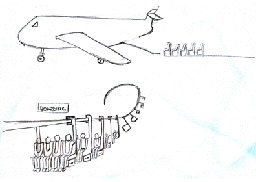
\includegraphics[width=7cm]{images/image007.png}
   \caption{Main themes driving our solution}
  \label{fig:main_themes}
\end{figure}

Our vision for a solution is a more dynamic cabin that allows the user to customize the space to his needs and allows for a more enjoyable and interactive experience.  If the world we live in is dynamic, then why does the airplane cabin have to be static with the same seating arrangements in all planes?  This is what we want to change.  We want to change the way a passenger looks at the flying experience and how they feel before, during, and after the flight.  The passengers should have more control over the seat selection, the firmness/softness of their seat, the angle, and the orientation; this list is endless. Giving passengers more independence and control while minimizing customer service interaction and discrimination is our motivation for a futuristic cabin that will make the entire air travel experience from home to gate to destination out of this world.

\begin{figure}[h]
  \centering
     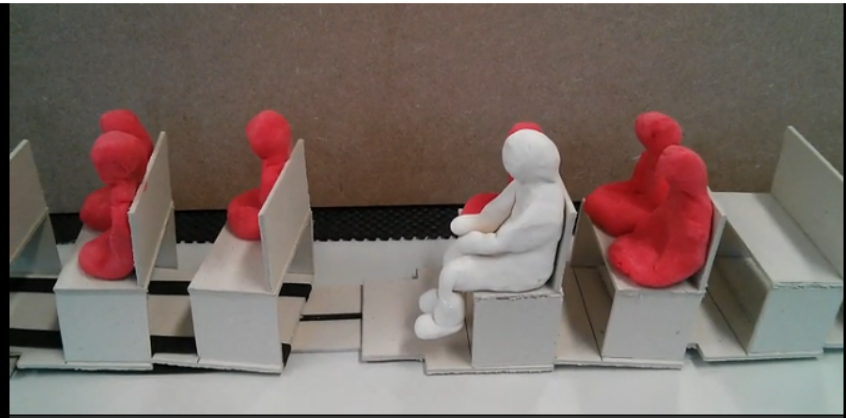
\includegraphics[width=7cm]{images/image008.png}
   \caption{Scaled mock-up of seats on rails prototype}
  \label{fig:mock_up_on_rails}
\end{figure}


\section*{Glossary}

\begin{list}{-}{}
  \item  \textbf{ADA:} Americans with Disabilities Act; one of America's most comprehensive pieces of civil rights legislation that prohibits discrimination against and guarantees people with disabilities have the same opportunities as everyone else to participate in the mainstream of American life.
  \item  \textbf{Assistive Technology:} Assistive, adaptive, and rehabilitative devices for people with disabilities; promotes greater independence by enabling people to perform tasks that they were formerly unable to accomplish, or had great difficulty accomplishing.
  \item  \textbf{Benchmarking:} A standard by which something can be measured or judged.
  \item  \textbf{CEP:} Otherwise known as a Critical Experience Prototype, this is a physical prototype created to make an experience “real enough” to gather insights and understanding about the user’s experience.
  \item  \textbf{CFP:} Otherwise known as a Critical Function Prototype, this is a physical prototype built to test a concept that is critical to addressing the problem statement.
  \item \textbf{Control:} The power to influence or direct either people's behavior or the course of events.
  \item \textbf{Dark Horse Prototype:} A device created during the winter quarter of ME310 that was ruled out in the fall quarter or undiscovered due to being “too risky” or “to difficult to complete”; emphasizes creative out-of-the-box thinking and exploring all of the design space for the project. 
  \item \textbf{Disability:} A physical or mental condition that limits a person's movements, senses, or activities.
  \item \textbf{FAA:} Federal Aviation Administration; United States national aviation authority whose mission is to provide the safest, most efficient aerospace system in the world, oversees all aspects of American civil aviation.
  \item \textbf{Herrmann Brain Dominance Instrument (HDBI):} Illustrates and explains the way a person prefers to think, learn, communicate and make decisions. It identifies the preferred approach to emotional, analytical, structural, and strategic thinking.
  \item \textbf{Independence:} Freedom from outside control or support.
  \item \textbf{Limited Mobility:} Mobility impairment may be caused by a number of factors, such as disease, an accident, or a congenital disorder and may be the result from neuro-muscular or orthopedic impairments. It may include conditions such as spinal cord injury, paralysis, muscular dystrophy and cerebral palsy. It may be combined with other problems as well (i.e. brain injury, learning disability, hearing or visual impairment).
  \item \textbf{Needfinding:} Discovering opportunities by recognizing the gaps in the system or the needs.
  \item \textbf{Non-Discriminatory:} Fairness in treating people without prejudice.
  \item \textbf{Pain Points:} A level of difficulty sufficient to motivate someone to seek a solution or an alternative; a problem or difficulty.
  \item \textbf{Perspective:} A particular attitude toward or way of regarding something; a point of view.
  \item \textbf{Self-Image:} The idea one has of one's abilities, appearance, and personality
  \item \textbf{ANAC:} Agencia Nacional de Aviação Civil – Brazilian National Agency of Civil Aviation
  \item \textbf{Libras:} Brazilian Sign Language
\end{list}


%%%%%%%%%%%%%%%%%%%%%%%%
% TOC and LOF are automatically generated -- Note that sometimes have to "compile" Latex THREE
% times to update the main .aux files, the TOC etc. files, and finally the PDF output with all changes
% propagated to the printout.
% Make Table of Contents title smaller than a normal Chapter heading:
\renewcommand{\chaptitlefont}{\normalfont\Large\bfseries}
\newpage
\tableofcontents*  %asterisk to prevent it from getting a number

% Optional Lists of Figures and Tables:
\newpage
\listoffigures*  %Note that for this you probably want to add the [short-headings] to captions.
%\listoftables  %I decided to omit the LOT in this example.

%Back to normal size for subsequent sections
\renewcommand{\chaptitlefont}{\normalfont\Huge\bfseries}
%%%%%%%%%%%%%%%%%%%%%%%%

% Set up the Glossary. The template is looking for a file called
% "glossaryterms.tex" with glossary terms and definitions.
% You can either edit this file manually or you
% can use the Memoir glossary feature in which you insert items like
%   \glossary{glossary term}{our definition of what the term means}
% wherever you like, as you write your documentation.
% When you run the report through Latex, it will create a ".glo" file like
% "OurFallDocument.glo" which you can edit to create the file "glossaryterms.tex"
% There is also perl script I made which will do the formatting for you. 
%  perl Glo2Tex OurFallDocument.glo > glossaryterms.tex
\newpage
\section*{Glossary}
\addcontentsline{toc}{section}{Glossary}
\label{sec-glossary}
\begin{description}
\begin{document}
\begin{list}
  \item  \textbf{ADA:} Americans with Disabilities Act; one of America's most comprehensive pieces of civil rights legislation that prohibits discrimination against and guarantees people with disabilities have the same opportunities as everyone else to participate in the mainstream of American life.
  \item  \textbf{Assistive Technology:} Assistive, adaptive, and rehabilitative devices for people with disabilities; promotes greater independence by enabling people to perform tasks that they were formerly unable to accomplish, or had great difficulty accomplishing.
  \item  \textbf{Benchmarking:} A standard by which something can be measured or judged.
  \item  \textbf{CEP:} Otherwise known as a Critical Experience Prototype, this is a physical prototype created to make an experience ��real enough�� to gather insights and understanding about the user’s experience.
  \item  \textbf{CFP:} Otherwise known as a Critical Function Prototype, this is a physical prototype built to test a concept that is critical to addressing the problem statement.
  \item \textbf{Control:} The power to influence or direct either people's behavior or the course of events.
  \item \textbf{Dark Horse Prototype:} A device created during the winter quarter of ME310 that was ruled out in the fall quarter or undiscovered due to being too risky or too difficult to complete��; emphasizes creative out-of-the-box thinking and exploring all of the design space for the project. 
  \item \textbf{Disability:} A physical or mental condition that limits a person's movements, senses, or activities.
  \item \textbf{FAA:} Federal Aviation Administration; United States national aviation authority whose mission is to provide the safest, most efficient aerospace system in the world, oversees all aspects of American civil aviation.
  \item \textbf{Herrmann Brain Dominance Instrument (HDBI):} Illustrates and explains the way a person prefers to think, learn, communicate and make decisions. It identifies the preferred approach to emotional, analytical, structural, and strategic thinking.
  \item \textbf{Independence:} Freedom from outside control or support.
  \item \textbf{Limited Mobility:} Mobility impairment may be caused by a number of factors, such as disease, an accident, or a congenital disorder and may be the result from neuro-muscular or orthopedic impairments. It may include conditions such as spinal cord injury, paralysis, muscular dystrophy and cerebral palsy. It may be combined with other problems as well (i.e. brain injury, learning disability, hearing or visual impairment).
  \item \textbf{Needfinding:} Discovering opportunities by recognizing the gaps in the system or the needs.
  \item \textbf{Non-Discriminatory:} Fairness in treating people without prejudice.
  \item \textbf{Pain Points:} A level of difficulty sufficient to motivate someone to seek a solution or an alternative; a problem or difficulty.
  \item \textbf{Perspective:} A particular attitude toward or way of regarding something; a point of view.
  \item \textbf{Self-Image:} The idea one has of one's abilities, appearance, and personality
  \item \textbf{ANAC:} Agencia Nacional de Aviação Civil – Brazilian National Agency of Civil Aviation
  \item \textbf{Libras:} Brazilian Sign Language
\end{list}
\end{document}   % input the list "glossaryterms.tex"
\end{description}

%%%%%% Example of an optionally printed "remark"
\begin{remark}
\color{blue}
It's a sign of a successful team that the glossary becomes extensive. Define any non-obvious or invented terms. For example, if you reference something by an acronym, that might be a glossary term. Teams also coin terms to describe design features. Define such terms here.  Don't define obvious stuff (axle, keyboard).  

See comments in me310report.tex if you want to generate a glossary semi-automatically from tagged keywords.
\normalcolor
\end{remark}


%%%%%%%%%%%%%%%%%%%%%%%%%%%%%%%%
%% On to the main sections....  Just comment out the \input{} line
%% for any chapters that aren't ready yet.

%%%%%%%%%%%%%%%%%%%%%%%%%%%%%%%%
%MRC5December2012 -- Added a bit about  the corporate partner context
%Context
\chapter{Context}
\label{sec-context} %Label for cross-referencing

\section{Need Statement}
Airlines are always searching for new ways to get more people on a flight and more money per flight, making the seats in the aircraft smaller and closer. As the seats get smaller, the personal space for a passenger shrinks, making it harder for anyone to move and fit comfortably as shown in Figure \ref{fig:1}.

\begin{figure}[h]
  \centering
     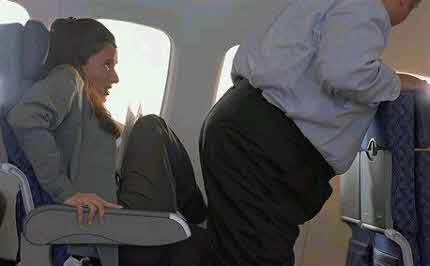
\includegraphics[width=7cm]{images/image009.png}
   \caption{With Airlines adding more and more seats to their planes, it is increasingly harder to maneuver around the cabin.
                  Source: http://www.examiner.com/article/airlines-may-charge-fat-people-higher-fares}
  \label{fig:9}
\end{figure}


With the emergence of global business, people are constantly on the go today and airports are becoming larger and larger, growing more busy each year.  The distance from check-in to gate is increasing as more airlines expand routes and terminals grow.  As the airports grow, it becomes harder to make the travel distance between check-in and gate short and quick.  Therefore, it becomes a problem for passengers that have a hard time walking long distances or need assistance with bags or a wheelchair. More airport staff is needed to move the passengers with assistance needs, and often the staff is not trained in dealing with disabilities.  Airlines have such limited space in the cabin because of the increased amount of seats that the assistive devices have to be stored in the cargo hold, making them susceptible to damage.  The flying experience today is tailored to a person that has all of his/her mobility, leaving out those who do not have the mobility or have some impairment that requires additional time. However, 58 million Americans live with a disability, including 5.5 million military veterans. \cite{}

Would it not be great if the flying experience were individually tailored to a person’s needs? What is the cabin could be redesigned to improve the flying experience for the passengers with limited mobility as well as for the average passenger? Such design would create an experience that is comfortable; making the airline and aircraft manufacturer more popular among its customers because the final user, the passenger, is the one the plane is designed for.

\section{Problem Statement}
To make this problem more tangible and approachable, we broke the project into different focus areas:

\begin{list}{-}{}
  \item Current systems in use in the airport and on the airplane
  \item User's Needs
  \item User'��s Complaints
  \item Identification of Critical Users
\end{list}

The whole process (see Appendix A�� Diagram A1) was analyzed and current systems that are in use based on FAA and ADA regulations were researched to determine the gaps in the system.  The gaps helped identify possible user needs.  In addition, user interviews were conducted to determine more needs and used to focus exact needs that we could address with our solution.  The interviews enlightened us with complaints that the current users had and ideas on where possible innovation areas lay.

For our problem, two distinct groups of users were quickly identified, the flight crew and the passengers with limited mobility.   The passengers with limited mobility were a very straightforward user group as it was identified in the problem statement.  However, the flight crew is the user that will have to use the solution on an everyday or every flight basis.  Therefore, the ease of use and the inclusion into the flight crew tasks have to be considered in order to make the solution a success.

\section{Corporate Partner: Embraer}

\begin{figure}[h]
  \centering
     
\includegraphics[width=7cm]{images/image010.jpg}
  \label{fig:10}
\end{figure}

The corporate partner for this design project is Embraer.  Since 1969, Embraer has been involved in all aspects of the aviation field.  Embraer began with support from the Brazilian Government to produce military aircraft in addition to its small passenger planes.  Embraer then expanded to agricultural planes and later to commercial planes and business/private jets.  Embraer has over 5,000 aircraft operating in over 80 countries.  They are the market leader for commercial jets with fewer than 120 seats.  Embraer is interested in expanding its commercial market to larger commercial jets, in maintaining some of the best executive jets, and in entering new defense markets.

\section*{Corporate Liaison}
Luciana Ribeiro Monteiro \\
  Technology Development \\
  Embraer - SJK \\
  Phone: +55 12 3927 8576 \\
  luciana.monteiro@embraer.com.br

\section{The Design Team}
Team Embraer was assembled using the results of the Herrmann Brain Dominance Instrument (HBDI) to determine compatible thinking styles and personality traits.  Additionally, our team has a diverse educational, cultural, and social background that encompasses many skill sets and multiple areas of study.

\subsection*{Stanford University}

\begin{figure}[h]
  \centering
     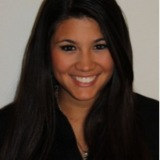
\includegraphics[width=7cm]{images/image011.jpg}
  \label{fig:11}
\end{figure}

\textbf{Maria Barrera}
Status: M.E. Graduate Student \\
Contact: mariab8@stanford.edu \\
I was born in Colombia and moved to South Florida with my mom when I was 10. My dad and sister still live in Colombia so I tend to hop back and forth every chance I get. I did my undergraduate at Stanford also in Mechanical Engineering and have developed a deep interest for entrepreneurship during my time here. I run a tutoring company in the area and hope to one day start a company in the aviation sector. I am also enjoy traveling, photography and playing with puppies.

\begin{figure}[h]
  \centering
     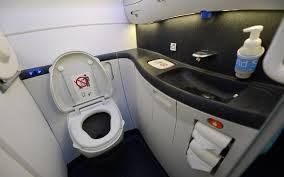
\includegraphics[width=7cm]{images/image012}
  \label{fig:12}
\end{figure}

\textbf{Erika Finley}
Status: M.E. Graduate Student \\
Contact: erikaf@stanford.edu \\
I was born and raised in Tennessee. I attended the University of Tennessee at Knoxville for my undergraduate degree in Mechanical Engineering.  I participated in a study abroad in Canberra, Australia.  I have interned for Tennessee Valley Authority at Browns Ferry Nuclear Plant and for Schlumberger at the Rosharon Design Center. I will be interning at Microsoft this upcoming summer. My interests include baking, reading, photography, and roller coasters.  

\begin{figure}[h]
  \centering
     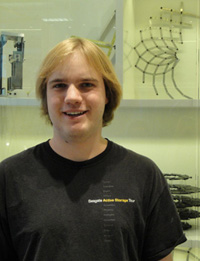
\includegraphics[width=7cm]{images/robert_karol.jpg}
  \label{fig:11}
\end{figure}

\textbf{Robert Karol}
Status: A.A. Graduate Student \\
Contact: robkarol@stanford.edu \\
I grew up in New Jersey through high school. After that, I moved to southern california where I attended the California Institute of Technology majoring in Mechanical Engineering with minors in Aerospace Engineering and Control and Dynamical Systems. I have worked on robotics projects with NASA's Jet Propulsion Laboratory, as well as experiments in high altitude photography and performed research in microgravity.

\subsection*{University of Sao Paulo}

\begin{figure}[h]
  \centering
     
\includegraphics[width=7cm]{images/image013}
  \label{fig:13}
\end{figure}

\textbf{Amanda Mota Almeida}
Status: Product Design Graduate Student \\
Contact: amandamotaalmeida@gmail.com \\
I was born and raised in São Paulo. I’m attending the University of São Paulo for my undergraduate studies in Product and Graphic Design. I have worked in a project with Embraer in the past regarding the design and comfort in the aircraft cabin (2011), I have interned for Staples in São Paulo – SP (2012) and I was part of exchange in Portugal last year (2013). My interests include: photography, arts and crafts and reading.

\begin{figure}[h]
  \centering
     
\includegraphics[width=7cm]{images/image014}
   \caption{With Airlines adding more and more seats to their planes, it is increasingly harder to maneuver around the cabin.
                  Source: http://www.examiner.com/article/airlines-may-charge-fat-people-higher-fares}
  \label{fig:14}
\end{figure}

\textbf{Rodrigo Monteiro de Aquino}
Status: Computer Engineering Undergraduate Student \\
Contact: guigonyts@usp.br \\
I have lived all my life in Sao Paulo. I am now graduating in Computer Engineering at USP and I also work in a technology development lab at the university. I have worked on several projects developing educational games and other educational interfaces that help children learn with technological devices.  I like to play videogames and go to the movie theater. I like science fiction movies and reading adventure books.

\begin{figure}[h]
  \centering
     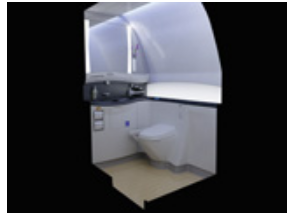
\includegraphics[width=7cm]{images/image015}
  \label{fig:15}
\end{figure}

\textbf{Luiz Durao}
Status: Industrial Engineering Undergraduate Student \\
Contact: luiz.durao@usp.br \\
I was born and raised in São Paulo city. I attended Colégio Etapa for my High School and it was while participating in the Chemistry and Physics Olympiads that I discovered my taste for the sciences. I'm attending the University of São Paulo for my undergraduate studies in Industrial Engineering. I have interned for GE Oil and Gas at Jandira – SP and I have worked since my sophomore year as a teaching assistant for some courses at USP. My interests include soccer, music and movies.

\begin{figure}[h]
  \centering
     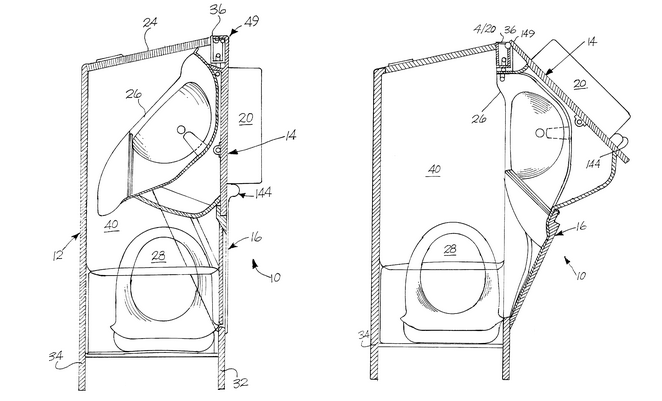
\includegraphics[width=7cm]{images/image016}
  \label{fig:16}
\end{figure}

\textbf{Guilherme Kok}
Status: Industrial Engineering Undergraduate Student \\
Contact: guilhermekok@gmail.com \\
Brazilian and a soccer enthusiast, I grew up in Sao Paulo and in Baltimore. I’ve also spent 5 months in Nanaimo (Canada, BC) and 1 year studying at the University of Illinois at Urbana Champaign. I’m currently finishing my undergraduate studies at the University of Sao Paulo in Brazil, where I study Industrial Engineering. I have interned for a taxi app startup and have done undergrad research concerning the consolidation of the phonographic industry. My interests include playing soccer, hiking, tasting different cuisines and travelling, preferably to remote locations. 

\section{Coaches}
a) Shelly Goldberg \\
Contact: shelly.goldberg@gmail.com \\ 
Shelly Goldberg was an ME310 alum from 2005, where her team worked on the EADS ?AugmenTable?.  Shelly has been at Apple, Inc. for the past 9 years since leaving Stanford.  She is now a Senior Manager in the Mac Product Design group, where she leads a team of mechanical and product design engineers responsible for conceiving, designing, engineering, producing, and sustaining the Mac portables and desktops.  

b) Annika Matta \\
Contact: annikamatta@gmail.com \\
Annika Matta is a former ME310 student and course assistant with a background in product and user experience design. As an ME310er she worked with SAP to build the Nib, a tablet with a writing experience reminiscent of paper. She graduated in 2013 and now works as a user interface designer at a consumer software startup in the Bay Area.
   %Your team, the corporate partner, the project background

%%%%%%%%%%%%%%%%%%%%%%%%%%%%%%%%
%%MRC5Dec2102 Added Venture Requirements suggestion.
%Design Requirements Chapter
\chapter{Design Requirements}
\label{sec-requirements}

\begin{remark} \color{blue}
Articulating design requirements is a critical task for a team that starts with a broad problem and needs to determine \emph{what they should design}. After need-finding, and technical and user benchmarking, the team proposes a {\em class of design solutions} that fulfill {\em requirements}\, associated with the problem. In the Fall document, the initial Requirements Definition is one of the first items of real value that teams can deliver to sponsors.

As the design process continues, requirements become more concrete and detailed. New {\em de facto} \, requirements are discovered and documented. Ultimately, competing designs are evaluated with respect to the requirements. If you can't tell whether a design satisfies the requirements, the requirements are too vague.


It is suggested to follow the procedure introduced in Fall quarter lectures and the Paper Bicycle Documents for defining and organizing requirements:\\
 \url{http://wikibox.stanford.edu:8310/12-13/Public/Fall2012-2013/Week2_2-4Oct/}

\normalcolor \end{remark}

%This table can  be copied & pasted in your document. The fussy formatting is already set up correctly.
%To get wrapped text, you have use p{} and specify paragraph widths (total < 148mm)
\begin{table}
\color{blue}
  \begin{tabular}{| p{44mm} | p{49mm} | p{42mm} |}   %3 columns, wrapped text
  \hline
  Requirement & Metrics & Rationale \\
  \hline
  \emph{What is the issue?} & \emph{What target values are we looking for?} & \emph{Why is this important?}\\
    \hline
  a brief description of what the requirement or objective is & 
  measurable quantities associated with requirement (how one knows if a design satisfies the requirement) &
  the  reasons why the it is important or valid \\

% This example table can be copied and pasted with the text adjusted to meet your needs. &
% Each column is separated by an ``\&'' sign. The text entries can wrap to more than one line if needed. &
% Each row is separated by two backslashes and an optional horizontal line. \\
    \hline
  \end{tabular}
\caption[Three column requirements format]{Three column format suggested for requirements (One can make a separate table for each cluster of related requirements).}
	\label{threecolumnreqs}  %Tag for referring to table
\normalcolor
\end{table}

\begin{remark} \color{blue}
The remainder of this section contains sample requirements (not an exhaustive set but enough to give an idea) from Autodesk Fall 2007-08 \cite{Autodesk2008Fall} and Audi Fall 2008-09 \cite{Audi2009Fall}.
\normalcolor \end{remark}

%%%%%%%%%%%%%%%%%%%%%%%%%%%%%%%%

\section*{Introduction}

The Autodesk collaboration tool must enhance communication between groups of distributed engineers as they engage in brainstorming.  We have focused on enabling this collaboration via tools that:

\begin{itemize}\tightlist
\item Enable users to communicate naturally and through multiple channels.
\item Enable the team to better utilize their teammates, be they local or distant.
\item Capture the information that was presented.
\end{itemize}

Our benchmarking and prototyping efforts have led to a more detailed definition of what the product needs to be in order to successfully achieve this.  The requirements address what the product functionally needs to do and what it physically needs to be. Because of the wide range of functional opportunities that exist for the product, few physical restrictions are imposed at this stage in the design. 

\section{Functional Requirements}
\label{sec:functionalreqs}

\begin{table}[!h]
	\centering
		\begin{tabular}{| p{42mm} | p{42mm} | p{51mm} |}
		\hline
		\textbf{Requirement}	& \textbf{Metrics} & \textbf{Rationale}\\
		\hline
The product will balance the number of interactions in distributed design meetings among the team members. &	Interactions are questions or statements that develop a concept. The total number of interactions per person during a design meeting will be called $n_{i}$. The solution must reduce the standard deviation of $n_{i}$ between team members as compared to the closest publicly-available competing product.	& The number of times someone interacts in a meeting is one measure of engagement. Brainstorming is a highly social process which thrives on the input from a variety of perspectives. By effectively improving the communication between distributed teams, team members will be more engaged and participate more.\\
\hline
		\end{tabular}
	\caption{Requirement for improved communication}
	\label{tab:mediums1}
\end{table}

\begin{table}[!h]
	\centering
		\begin{tabular}{| p{42mm} | p{42mm} | p{51mm} |}
		\hline
		\textbf{Requirement}	& \textbf{Metrics} & \textbf{Rationale} \\
		\hline
The solution must transmit sound at close to the rate of normal conversation. &	The listener must hear the speaker with less than 0.3 seconds lag.	& Audio latency creates a sense of distance. Mobile phone to mobile phone conversations have an average latency of 0.3 seconds, which is noticeable but not disruptive. \\ \hline
Users can capture drawings to share with distributed teammates that are legible. &	Input device must be able to resolve a drawing at 50 points per inch (specifically, they must capture 50 percent contrast modulation at this frequency). &	Drawings by mechanical pencil and ball point pens typically have lines of 0.5mm thickness, which translates to a resolution of 50 points per pinch (ppi).\\ \hline
Users will be able to capture drawings to share with distributed teammates without disrupting the flow of the discussion. & Drawings must be captured and sent within 17 seconds. This is assuming the input device is properly set and there are no external complications. &	We found through benchmarking that sketches are used primarily when describing a concept, and are of little use afterwards. The sketches must be captured and sent before the context of the discussion has changed. Seventeen seconds was found to be about the average comment length during brainstorming in our prototyping. \\ \hline
Users will be able to see the drawings clearly. &	Drawings must be displayed with a resolution of at least 72 ppi.&	The display must be able to resolve at least as a standard computer monitor.\\ 
\hline
		\end{tabular}
	\caption{Required mediums of communication for effective concept development}
	\label{tab:mediums2}
\end{table}

\begin{table}[!h]
	\centering
		\begin{tabular}{| p{42mm} | p{42mm} | p{51mm} |}
		\hline
		\textbf{Requirement}	& \textbf{Metrics} & \textbf{Rationale} \\
		\hline
The tool must be able to be started up quickly for impromptu meetings.	& It must be able to be started in less than 40 seconds. This time is calculated from the moment someone decides to start the system, to the point when the tool is ready to use, with full functionality. If the solution requires use of personal laptops, assume these are already booted up. & Our benchmarking has shown that collaboration tools can fall into disuse if it requires a lengthy setup time. This amount of time is within the range of initiation times for multiple popular conferencing solutions. \\ \hline

	\end{tabular}
	\caption{Social requirements for effective design meetings}
	\label{tab:mediums3}
\end{table}



\newpage

\subsection{Functional constraints}

\begin{table}[!h]
	\centering
		\begin{tabular}{| p{44mm} | p{49mm} | p{42mm} |}
		\hline
		\textbf{Requirement}	& \textbf{Metrics} & \textbf{Rationale} \\
		\hline
		The bandwidth required must not be prohibitive to standard engineering offices.	& The product will require less than 100 Mbps.& The population of potential users would dramatically decrease if the product required more connectivity than a T1 line, which is typically around 100 Mbps.\\ \hline
			\end{tabular}
	\caption{Functional constraints}
	\label{tab:fconstraints}
\end{table}


\subsection{Opportunities}

\begin{itemize}\tightlist
\item Utilize existing tools. There are many collaboration and input  tools that exist out there. Our product does not need to be a replacement for them. It could potentially supplement them.
\item Offer new lines of communication:
	\begin{itemize}\tightlist
 		\item Facilitate side conversations between distributed users.
 		\item Utilize the uncrowded channels offered by other senses than audio/visual, such as tactile.
\end{itemize}
\newpage
\item Be the moderator: 
\begin{itemize}\tightlist
 		\item Collect feedback from users directly, via voting, or indirectly. Enable the replacement of video, which conveys very little useful feedback during design meetings.
		\item Encourage the participants to be engaged by monitoring participation.
		\item Display feedback and participation to attendees non-verbally,potentially through the use of avatars.	
\end{itemize}
\item Allow for easier information capture and storage
\begin{itemize}\tightlist
 		\item One button information capture
		\item User-driven archiving
\end{itemize}
\item Assist user communication in non-native languages.
	\begin{itemize}\tightlist
 		\item Audio buffering
 \end{itemize}
\item The product should be accessible
\begin{itemize}\tightlist
\item Usable for low bandwidth connections for 
\item Be fast to setup.
\item Able to be setup within a typical conference room.
\end{itemize}
\end {itemize}

\subsection{Assumptions}
\begin{itemize}\tightlist
\item Each user has, and is able to use:
\begin{itemize}\tightlist 
\item a personal laptop
\item a mouse
\item a microphone
\end{itemize}
\item Users will speak with a volume of at least 30 dB, as measured when 1 meter from the microphone.
\end{itemize}

%%%%%%PHYSICAL REQUIREMENTS%%%%%%%%%%%
\section{Physical requirements}
\label{sec:physicalreqs}

\color{blue}
For variety, here is a requirements table from an Audi fall document \cite{Audi2009Fall} done in MS Word and pasted as PDF into Latex. Notice that the fonts are scalable if you zoom in.
\normalcolor

\begin{table}[h]
	\centering
		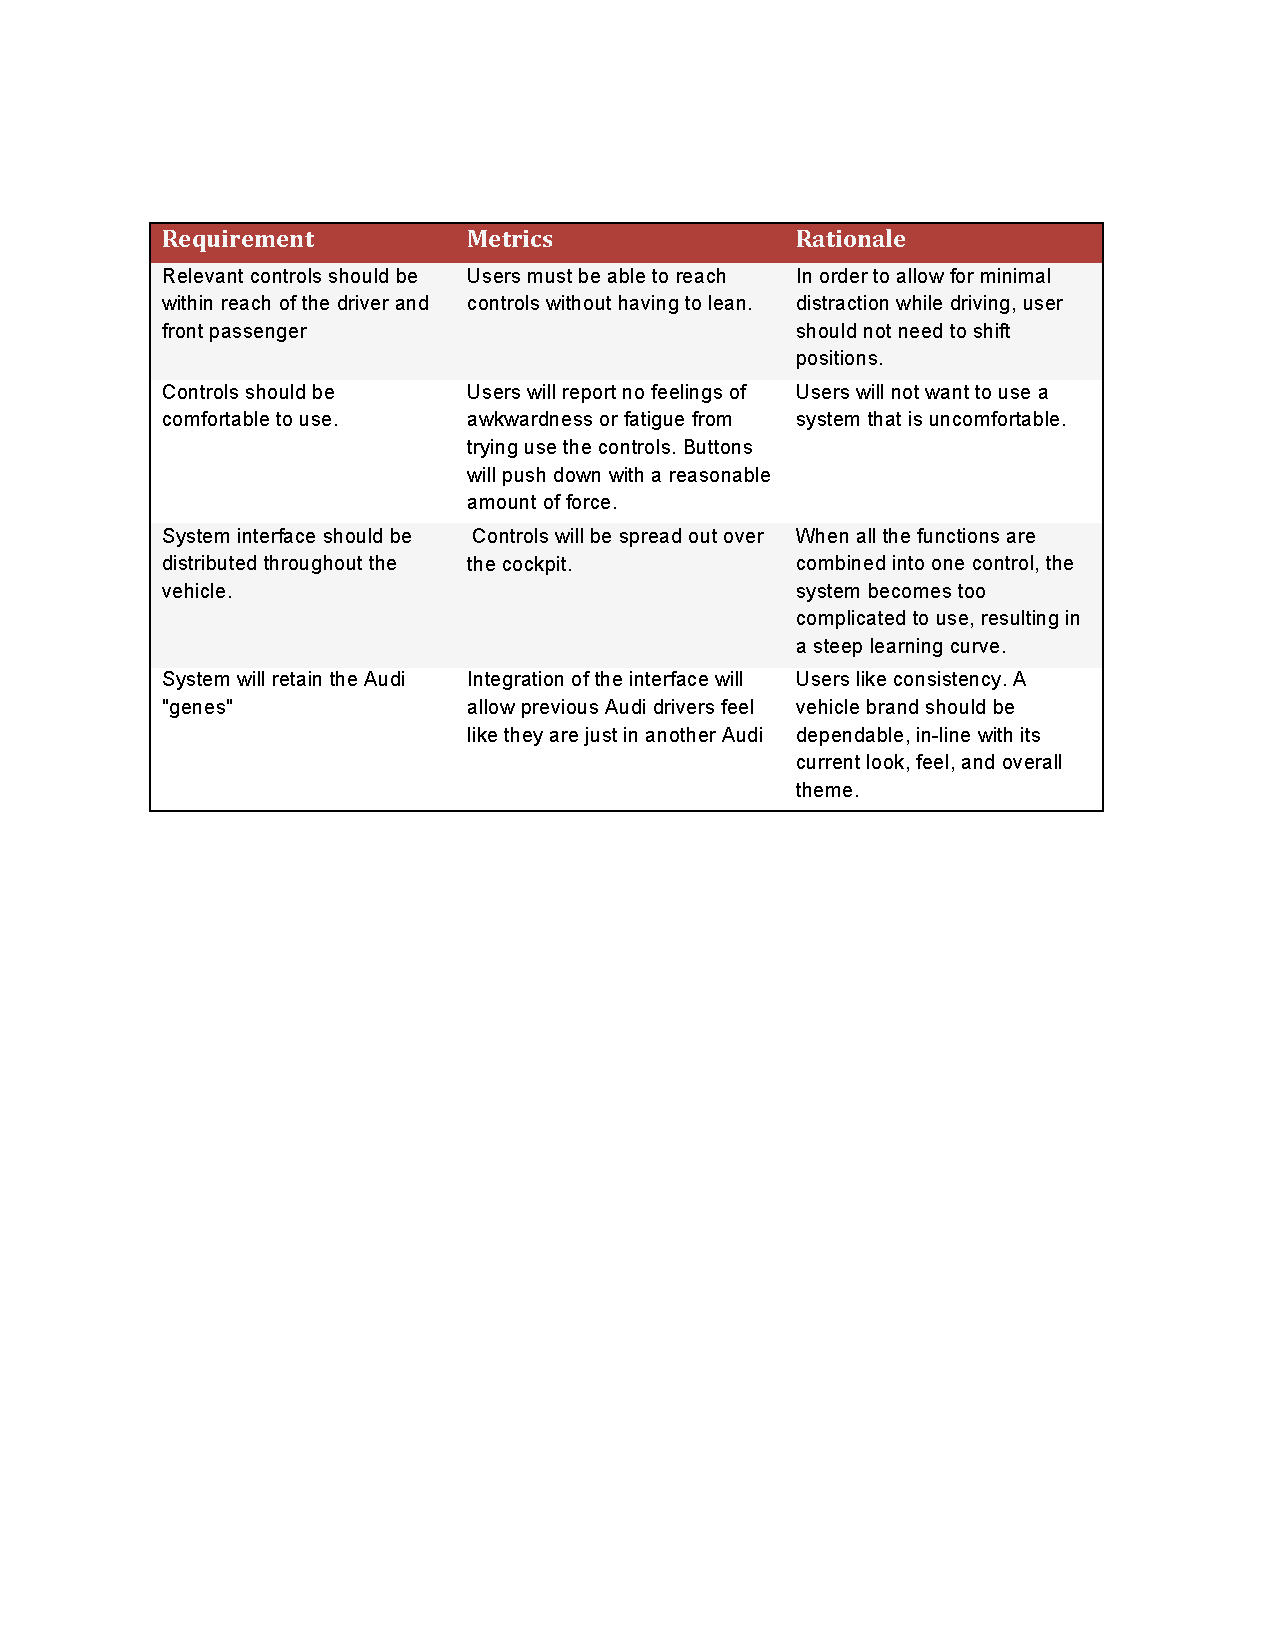
\includegraphics[width=\textwidth]{Figures/Ch3/Audi08PhysReqs.pdf}
	\caption{Physical Requirements from Audi 2008-09}
	\label{tab:physical-requirements}
\end{table}

\subsection{More physical requirements}
\label{sec:morephysical}

\color{blue}
Here is an example of a Physical Requirements table from a spring document. The 4th column is probably not appropriate for Fall. This example is include to show how one can make a long table that spans multiple pages.
\normalcolor

%%Example of a long  table using supertabular and tablefirsthead
%%
\begin{center}
\tablefirsthead{%
\hline
\textbf{Requirements} & \textbf{Metric} & \textbf{Rationale} & \textbf{Requirements met?}\\
\hline}
\tablehead{%
\hline
\multicolumn{4}{|l|}{\textit{\small{continued from previous page}}}\\
\hline
\textbf{Requirements} & \textbf{Metric} & \textbf{Rationale} & \textbf{Requirements met?}\\
\hline}
\tabletail{%
\hline
\multicolumn{4}{|l|}{\textit{\small{continued on next page}}}\\
\hline}
\tablelasttail{\hline}
\bottomcaption{This physical requirements table is from a spring document to show splitting across pages and addition of a 4th column regarding whether design meets the requirements}
\begin{supertabular}{| p{32mm} | p{37mm} | p{33mm} | p{33mm} |}
\hline
Use limited force to activate mechanical mechanism(s) & Force required for activation is {\textless} 20 N & User should be able to operate system without excessive force & The design should fulfill this requirement, however final gas spring and seat securer installation and thereafter testing will confirm this\\
\hline
System is ergonomic & User should be able to operate all mechanisms 4 times in the span of 1/2 an hour without any serious exertion (no sweating, strained breathing, or muscle soreness) and should be able to use the system for 2 hours without muscle cramping or other physical afflictions & System should be physically comfortable to use for a long commute time & User testing needs to be performed; initial prototyping seems to show this is satisfied\\
\hline
System is durable and robust & Lasts at least 2 years of daily use and its structure cannot be significantly altered by an average man or woman applying a full impact force on structural elements of the module & As part of a PT system, all modules should be resistant to daily use by an average human and vandalism & Robust materials such as steel and actual public transport-quality seats and flooring has been used; needs to be tested\\
\hline
Parts can be easily replaced and easy to maintain, including easily cleaned and water resistant & Takes no more than 5 min for one person to replace parts of a single module; module can be fully cleaned in 15 minutes; module shows no signs of corrosion over its 2 year life span & PT parts see significant wear and it should be convenient to replace modules as necessary & Needs to be verified\\
\hline
Seat is comfortable & Seat is breathable (from fully soaked takes {\textless}15 to air dry) and has a high thermal conductivity (seat adjust to room temperature from a 20-degree difference in less than 5 minutes) & Commuter should have a pleasant commuting experience while seated & Good quality seats of actual public transportation quality have been procured and used\\
\hline
Module should be safe & There should be no pinch points, sharp points, or possibilities for latches or other physical mechanisms to fail & System should not cause any users bodily injury & Mechanisms have been designed to avoid pinch points; final verifications needed\\
\hline
System should be aesthetically pleasing & At least 80\% of surveyed users should react positively to the device forms & A pleasing system will encourage adoption and use & Visual language was established earlier on in the design phase; final aesthetic styling still needed upon final integration\\
\hline

\end{supertabular}
\end{center}

\section{Business requirements (or Venture requirements)}
\label{sec:venturereqs}

A new element in me310-global thinking for 2012-13 is to be more aware of the client�s business model.  This is not so much about designing a new business model as it is about business context awareness.  The main discussion of this business model belongs in chapter \ref{sec-development} as part of your benchmarking. Here is where you could note any particular requirements or ramifications  that it has for your design.






%This section is omitted from the Fall document

%%%%%%%%%%%%%%%%%%%%%%%%%%%%%%%%
% Design Development 
\chapter{Design Development}
\label{sec-development}

For fall, the development chapter focuses on benchmarking, need-finding, persona development and the first critical function and critical experience prototypes. For later quarters, many of these details will go to an appendix, with just a summary of the main findings and insights. Even in fall, the focus should be on findings and lessons learned.

\begin{remark}  \color{blue}
\begin{itemize}\tightlist
\item Focus on results (e.g., key findings, insights, lessons learned), not team activities (``We brainstormed extensively and eventually settled on two alternative concepts.'')
\item Use lots of images, and not just photographs: diagrams, schematics, flow charts, CAD renderings, etc. are often much more informative than a photo. In any case, use labels pointing to the features you want the reader to appreciate. Also, do refer to all of your figures explicitly in the  text (\emph{As shown in figure xx, ... }).
\item Lengthy details (e.g. detailed results of technical benchmarking) should go in an Appendix section, with an explicit forward reference from this section. In winter and spring, much of this material will go to an appendix.
\item Be professional: it's essential to properly cite sources of information and provide credits for any images you are using that you did not generate yourselves.
\item Don't refrain from describing ideas that were briefly pursued and dropped. Explain why they were abandoned. In other circumstances they might be worth picking up again.
\item You can use tools such as Pugh concept selection, function-structure diagrams and design decomposition 
\cite{Otto07,OttoWood01,UlrichEppinger95} to organize and clarify your design process. Many web-based tools also exist for diagramming relationships (e.g. \url{http://vue.tufts.edu} ). A nice side-effect is that such diagrams help with documentation.
\end{itemize}

The remaining text in this section contains excerpts from the Autodesk 2007-08 Fall document \cite{Autodesk2008Fall} and some additional explanatory examples.
\normalcolor 
\end{remark}

We drew from our diverse individual experiences to redefine the problem as we learned more about existing collaborative tools and practices. Throughout the design development process, shown in figure \ref{fig:Design_Development_Flowchart}, we balanced pushing forward with our current ideas while looking for new directions. 

\begin{figure}[h]
\centering
		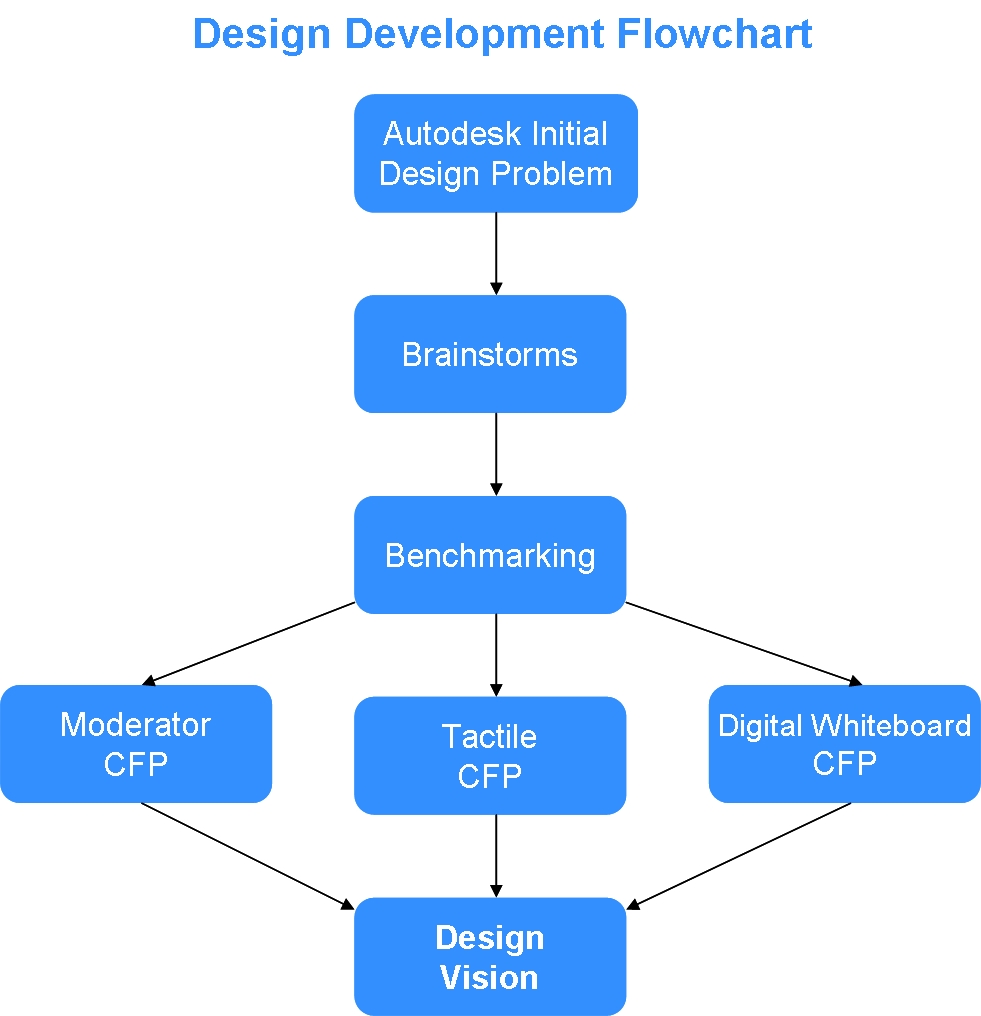
\includegraphics[keepaspectratio, width=4in]{Figures/Ch4/Design_Development_Flowchart.jpg}
	\caption{The design team's development process.}
	\label{fig:Design_Development_Flowchart}
\end{figure}

\section{Brainstorming}
\label{sec:brainstorm}

	Our experience in brainstorming was unique in that we were observing and studying our own behavior while exploring solutions. We were constantly studying our own triumphs and shortcomings in the hopes of gaining insight into team dynamics. The results of our multiple brainstorms throughout the fall quarter can be into categorized the following categories:

\subsection{Communication}

\begin{figure}[h] 
\centering
		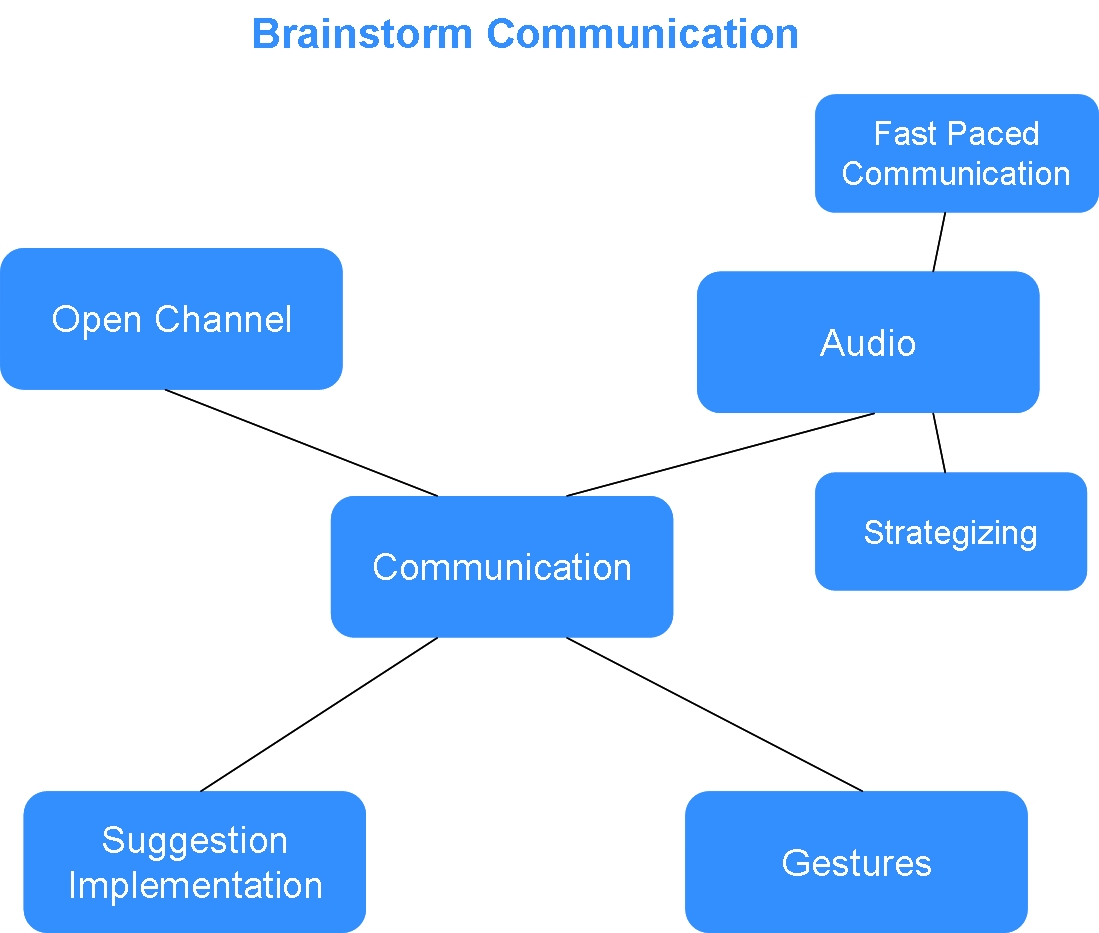
\includegraphics[keepaspectratio, width=3in]{Figures/Ch4/Brainstorm_Communication.jpg}
	\caption{Key components of communication in design meetings}
	\label{fig:Brainstorm_Communication}
\end{figure}

\begin{itemize} \tightlist 
\item {Open channels}
\item \begin{itemize} \tightlist Audio and video channels are often inundated with information, even if they are not the most effective means to transmit a piece of information. The team learned that messages are most clearly conveyed when they are free from interference. \end{itemize}
\item Integrate suggestions quickly
\item \begin{itemize} \tightlist People can build onto other's ideas immediately, and rapidly change the direction of the conversation. \end{itemize}
\item \textbf{Verbal communication is the most flexible}
\item \begin{itemize} \tightlist The team learned from their experience playing cutting-edge multiplayer videogames that verbal communication was the most relied upon medium during fast and slow paced activities. It's versatility and low-bandwidth warranted future attention. \end{itemize}
\item Gesture
\item \begin{itemize} \tightlist Gesture is frequently used when explaining an idea. Often, the drawings produced do not look at all like the concept being developed, but the act of drawing in and of itself can be like a gesture, showing how something will work, or where it will be placed, and so forth. \end{itemize}
\end{itemize}

\begin{center}
\emph{The rest of this subsection is omitted for brevity}
\end{center}

Some key realizations from the brainstorming phase were that social factors and communication shortcomings had alot of opportunity for development. We decided to give special attention to social benchmarking in addition to our technological research.

\section{User benchmarking and need-finding}
\label{sec:needfinding}

In this section briefly describe activities undertaken to come to an understanding of users or potential users and their needs. An important part of this section is the development of personas.

\subsection{Personas development}
\label{sec:personas}

Describe the personas, what findings are incorporated in them, and what insights they provide for the design.  Ideally include some images of your personas, like ``Kevin'' in figure \ref{fig:personakevin} from the 2011 Lockheed project \cite{LockheedMartin2011}.

\begin{figure}[h]
\centering
		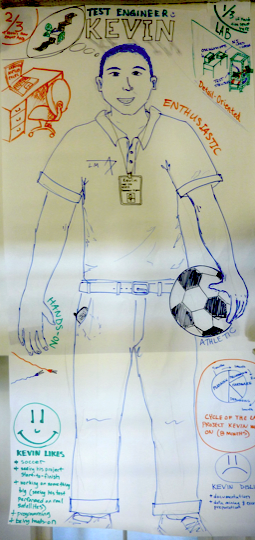
\includegraphics[keepaspectratio, width=2in]{Figures/Ch4/persona-kevin.png}
	\caption{A persona for a satellite testing project (from \cite{LockheedMartin2011})}
		\label{fig:personakevin}
\end{figure}

\section{Business Benchmarking}

A recent element in me310-global thinking process is to be explicitly aware of the client's business model.  
The motivation for this new element is our growing awareness that coming up with the next ``big-idea'' may be the easy part of our quest.  The harder part may be gaining acceptance of our break-through innovation within the organization. 
Please be aware that the canvas can be re-organized to suit your situation. 

A starting point could be the ``Business Canvas Model''
introduced in class (figure \ref{fig:businesscanvas}) with reference to
\cite{osterwalder2010business} for more background information.

Bencharking the corporate partner's business model and goals is part of benchmarking, and can be covered in a section 
in this design development chapter. Some examples of recent ME310 documents with fairly extensive business
benchmarking include the 2012 Spring documents from Electric Mobility Norway \cite{EMN2012Spring} and Symbiose\'{e} \cite{Symbiosee2012Spring}.

\begin{figure}[ht]
\centering
		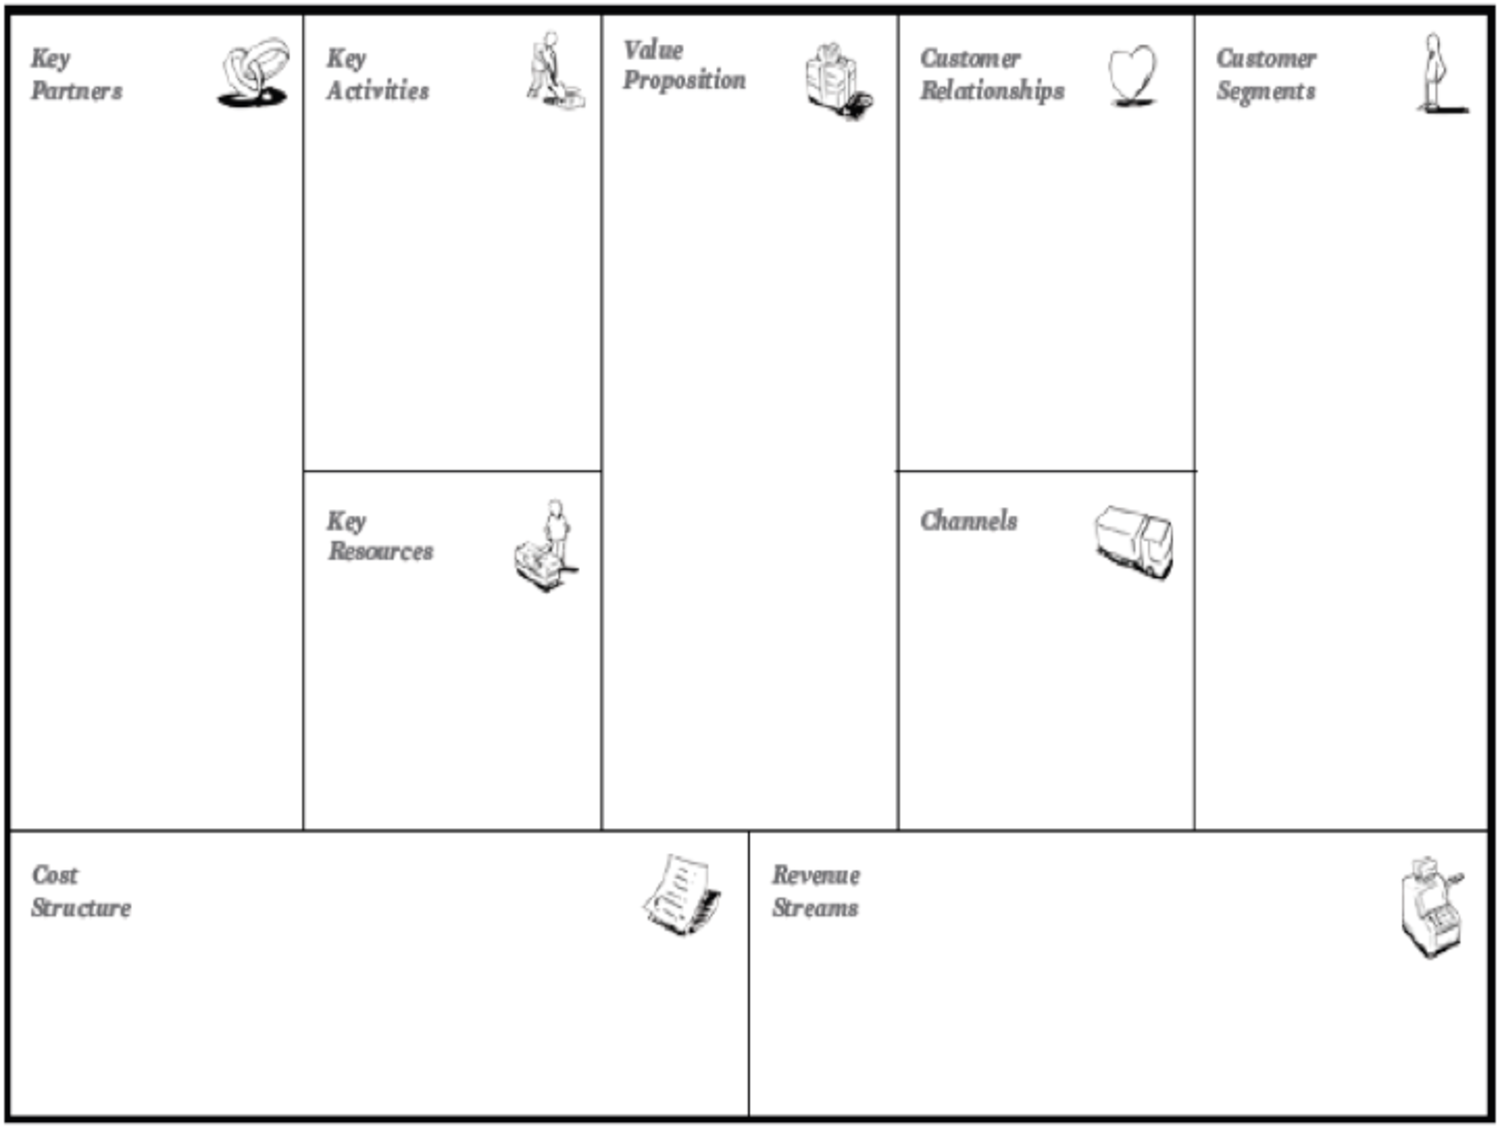
\includegraphics[keepaspectratio, width=4in]{Figures/Ch4/BusinessCanvas.pdf}
	\caption{Business Canvas (from \cite{osterwalder2010business}).}
		\label{fig:businesscanvas}
\end{figure}


\section{Technology benchmarking}

	The team's research and benchmarking efforts were focused on three major categories: human-machine interfaces and input devices, social dynamics, and communication. The methods the team utilized to research items in these three main categories  included trying out hardware, drawing on previous experience, participating in improv exercises, researching existing solutions, and speaking to experts from design, neuroscience, and computer science.
	
\subsection{The Nintendo Wii - Accelerometer-based input)}

\begin{figure}[h] 
\centering
		\includegraphics[keepaspectratio, width=4in]{Figures/Ch4/Wii.jpg}
%Note the use of a short caption tag for the list of figures.
	\caption[Nintento Wii]{People playing Wii Sports on the the Nintendo Wii.
	\color{blue}There should be a citation to the URL this photo came from\normalcolor. }
\end{figure}

	The team investigated some unconventional means for data input. Gesture-based input devices like the Nintendo Wii controller offer the possibility of an intuitive, and compelling way to interact with someone at distance via digital means.  For navigating through Windows or other applications, the team found the Wii to be  more challenging than a conventional mouse.  Accelerometers are adept at capturing large motions rather than precision pointing and would need to be utilized as such. Potential applications could be for interfacing with avatars or tactile feedback systems. The Wii controller could be used as a gesture-based communication device to control a personal avatar or send and receive tactile messages.
	
\noindent \textbf {Key lessons learned}
\begin{itemize} \tightlist 
\item Accelerometer based input devices could be used in gesture-based or tactile communication, but do not fare well in precision pointing.
\item Gesture-based interfaces generate excitement. People want to use input devices that respond to gesture. 
\end{itemize}

\subsection{CyberGlove \textregistered}

\begin{figure}[h] 
\centering
		\includegraphics[keepaspectratio, width=4in]{Figures/Ch4/CyberGlove.jpg}	
%Note the use of a short caption tag for the list of figures.
	\caption[Cyberglove]{CyberGlove gesture-based input device. \color{blue}There should be a citation to the URL this photo came from\normalcolor.}
\end{figure}

\begin{center}
\color{blue}
The rest of this subsection is omitted for brevity
\normalcolor
\end{center}

\subsection{EEG and Participation Monitor}

\begin{figure}[h] 
\centering
		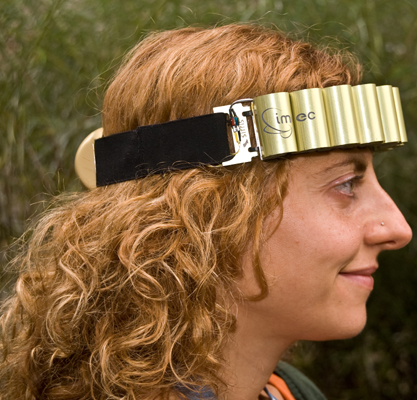
\includegraphics[keepaspectratio, width=3in]{Figures/Ch4/EEG.jpg}
	\caption[Wireless EEG]{Example of the first available wireless EEG tool, made by IMEC. \color{blue}There should be a citation to the URL this photo came from\normalcolor.}
\label{fig:wirelessEEG}
\end{figure}

	The team met with Alicia Warlick, a researcher in the Stanford Neuroscience Department, and her research in monitoring brainwaves. We discussed the possibility of monitoring whether meeting participants were actively paying attention by using an EEG. This is a method for measuring the activity level of the brain. There is opportunity to use this as a metric for testing our final product, or potentially in the product itself as a means to collect data on user participation level.

\noindent \textbf{Key lesson learned}
\begin{itemize} \tightlist
\item  Electrodes could be placed on the users forehead and scalp (as in Fig. \ref{fig:wirelessEEG}) to measure EEG readings, which conveys information about whether someone is engaged in what they are doing, or if they are withdrawn.
\end{itemize}

\begin{center}
\color{blue}
The rest of this subsection is omitted for brevity
\normalcolor
\end{center}

%%%%%%%%%%%%%%%%%%%%%%%%%%%%%%%%%%%%%%%%%%
%This starts a major new subsection on the final CFP and CEP of Fall quarter, so
%probably makes sense to put in a clearpage command to let figures catch up.
\clearpage

\section{Critical Function and Critical Experience Prototypes (CFP/CEP)}
	The initial benchmarking phase lead the team to realize that there were three major challenges to solve: bridging the proximity gap, moderating brainstorming, and conveying and recording ideas. The team decided to tackle all three of these major challenges and designed four CFPs in an attempt to solve, or at least start answering some of, the questions these challenges brought up. 

\subsection{Tactile CFP}

The team wanted to come up with a creative solution that would enhance distance communication. Although we identified software having an important role in our solution, we wanted to try to design something physical. We had to answer these questions that were raised after the benchmarking process:
\begin{itemize} \tightlist
\item How can we simulate proximity for remote meetings?
\item How can we implement action-event control?
\item What senses can we stimulate that aren't normally used?
\item What is a low bandwidth solution?
\end{itemize}

	The team decided that building a tactile messaging system would solve all four of the aforementioned questions. Tactile messages could replace common interpersonal interaction found in same room meetings. It is normal to welcome each other with a  handshake, make eye contact throughout a meeting, smile at each other, and give high-fives to congratulate others. These occurrences are all absent from distance meetings. A tactile message corresponding to each of these gestures would allow users similar opportunity to communicate as if they were sharing the same physical meeting room.
	
	The team learned that immersive activities like videogames take advantage of action-event control to offer users a seamless means to interact with their environment. A tactile message could quickly be sent over an open channel and pressing the �on� button would instantly message the recipient.
	
	Out of the five senses (sight, hearing, taste, touch, and smell), sight and hearing are the most relied upon during meetings. The team considered possibilities in taste and smell messaging but continued with touch, since delivery of tactile messaging was much more straightforward. Since conventional distance meetings only send and receive auditory and visual information, tactile messages would be distinct and easy to identify. The team believed that tactile messages (high, low, or off) would be low bandwidth.

	\begin{figure}[h] 
\centering
		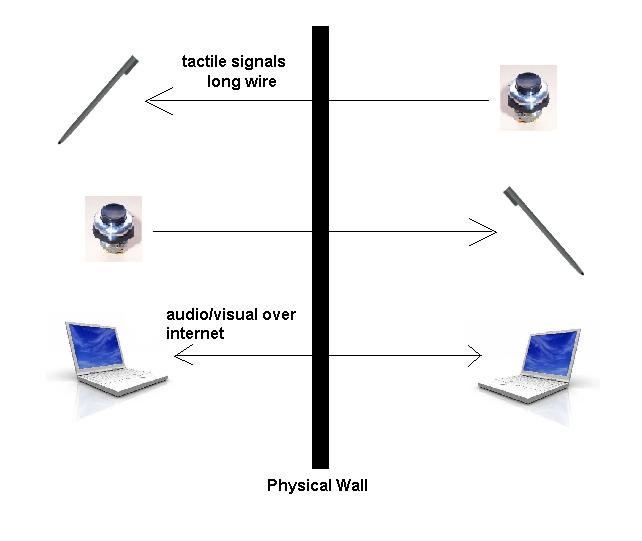
\includegraphics[keepaspectratio, width=4in]{Figures/Ch4/tactileCFPschematic.jpg}
	\caption{The team's whiteboard during a brainstorm session}
\end{figure}

	The team wanted to test the effectiveness of tactile messaging and decided against a TCP/IP protocol that sent messages between Stanford and PUJ. The code to write such a protocol was extant and it was unnecessary to include it in our prototype. The team simplified the setup and created two stations separated by physical barriers (a wall and 50' of distance), to simulate a distance meeting. Each station would have a vibrating tactile device for each seated participant at that station and a high/low button assembly to activate the vibrating tactile device for each participant at the other station. Initially the devices were supposed to operate as ''on'' or ''off.'' The team decided that having more variability in the operating speeds of the motors would increase the number of different messages that could be sent, and added a high and low voltage button (1.2V and 0.6V).
	
	We were curious to see if effective communication could take place if a distant colleague could see what sketches his distant colleague was drawing. To test this, we used webcams to send live video of what the participants drew on their drawing pads to the other stations.

\subsubsection{What is critical about this CFP?}
	The team identified these questions as critical before testing:
\begin{enumerate} \tightlist
\item Can it create immersion?
\item Does it improve upon existing communication tools?
\item Is it easy to understand?
\item Is it intuitive?
\item When should it be used?
\end{enumerate}

\begin{figure}[h] 
\centering
		\includegraphics[width=3in]{Figures/Ch4/tactile_seating.jpg}
	\caption{The orientation of the two tactile messaging stations.}
\end{figure}

\subsection{Tactile Messaging CFP Description}

The remaining text in this section contains of excerpts from the Autodesk 2007-08 Fall document \cite{Autodesk2008Fall}.

The tactile messaging system was comprised of small Jameco vibrating motors (1.3VDC 8,500 RPM) mounted to ball point pens and wrist patches. A simple switchable voltage supply circuit was created to give each vibrating motor a high (1.2V) and low (0.6V) vibrating speed (\ref{fig:tactile_circuit}). Each voltage level was buffered with LM324 opamps, and the circuits were implemented on protoboards. The high and low speeds were selected by switches. 

\begin{figure}[bhtp] 
	\begin{center}
		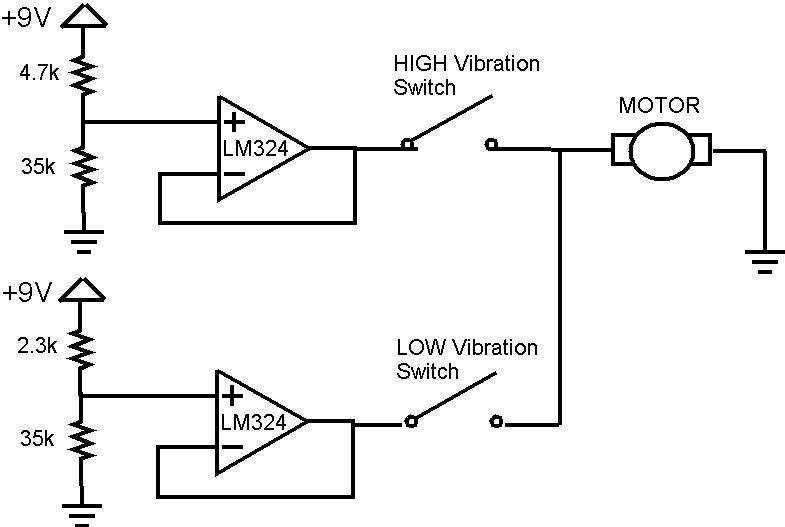
\includegraphics[width= \figwidth]{Figures/Ch5/tactile_circuit.jpg}
	\end{center}
	\caption[voltage divider]{A simple voltage dividing circuit provided 1.2V (HIGH) and 0.6V (LOW) buffered output voltages for the vibrating motor. Switches triggered the high and low voltages. }
	\label{fig:tactile_circuit}  
\end{figure}

\begin{center}
\color{blue}
(Text omitted for brevity)
\normalcolor
\end{center}

Four independent circuits were created to provide messaging to two motors on each side. 90' 16-gauge wire was passed between two stations in the meeting setup shown in \ref{fig:tactile_seating}. Power supplies provided the 9V signal on each side.

\begin{figure}[bhtp] 
	\begin{center}
		\includegraphics[width=3in]{Figures/Ch5/tactile_seating.jpg}
	\end{center}
	\caption[test meeting layout]{Layout of seating during test meeting. Two participants met on one side, with the remote user separated by a wall 50 ft away. }
	\label{fig:tactile_seating}  
\end{figure}

In addition to the tactile hardware, Skype was used for video and audio communication. Video was supplied by standard webcams. We mounted the webcams on risers to show video of a sheet of white paper used as the shared drawing space. We chose to focus the video on ideas rather than facial expressions. 


\clearpage
\subsection{Moderator CFP Description}

\subsubsection{Layout}

The participation moderator was created by using pre-made desktop software applications called widgets. The desktop was set to a white image, with personal spaces for each participant mapped off by a black boundary and labelled with the participant name. In each personal space, a unique Yahoo! Widgets timer was placed. Unique timer's were used to foster a sense of identity- when glancing at the moderator, the team members could instantly recognize their widget rather than look for their name. 

\begin{figure}[htbp]
	\centering
		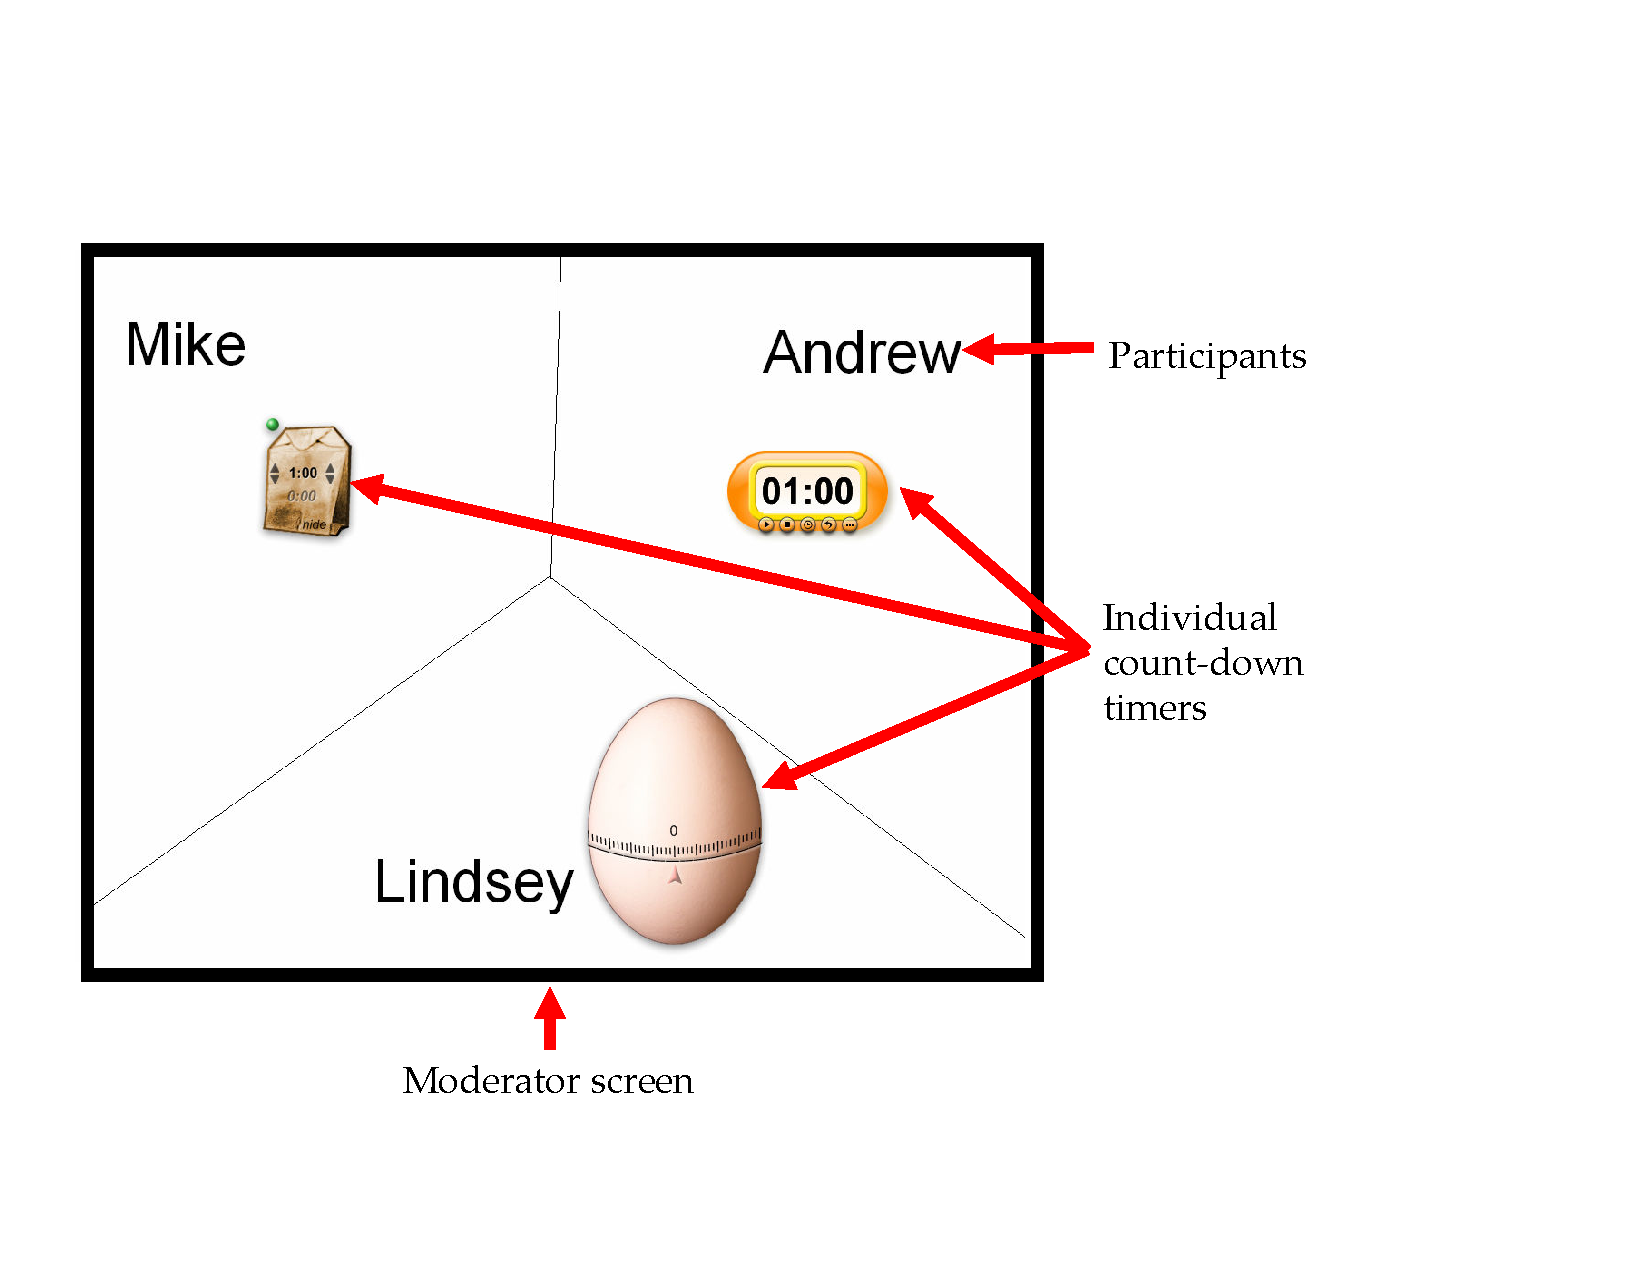
\includegraphics[width=1.00\textwidth]{Figures/Ch5/moderator.pdf}
	\caption{View of moderator display}
	\label{fig:moderator}
\end{figure}

\begin{center}
\color{blue}
(Text omitted for brevity)
\normalcolor
\end{center}


Each was simply a countdown timer with a default starting time, $t_{s}$. As they begin counting down, the amount of time remaining is visible. By clicking twice on any widget, it would reset and begin counting down again from $t_{s}$. The timers were manually reset by one of the teammates during the meeting whenever someone had an interaction. When any timer runs out, it would sound an alarm, designating that the meeting come to a halt until the non-active team member contributes to the conversation. The hypothesis was that, because the timers were visible to the entire team, each member would consciously make an effort to speak before their timer ran out and that no timer would actually buzz, although the rotation of speakers would greatly increase.

The moderator screen was displayed on a 32" LCD display that was positioned 6' from the center of a table where the group met. The layout is detailed in Figure \ref{fig:moderator_setup}. No video or audio conferencing was used -- all team members were local. The objective of the moderator is to support dialogue in meetings, regardless of whether the members are distributed or not. Audio was recorded of each meeting using Cubase software and an IBM laptop's internal microphone, which was placed in the center of the table so each participant could be heard. 

\begin{figure}[h]
	\centering
		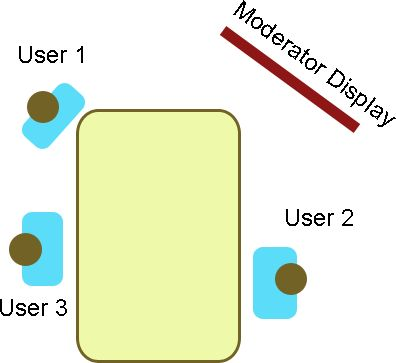
\includegraphics[width=.75\textwidth]{Figures/Ch5/moderator_setup.jpg}
	\caption{Layout of design meeting with moderator prototype}
	\label{fig:moderator_setup}
\end{figure}

\subsubsection{Procedure}

Three meetings were run to test the moderator. The subject of each was the same - our team brainstormed potential final products knowing the key lessons learned after our benchmarking. Three meetings were run in succession, each lasting 30 minutes. The intention of this was to eliminate any personal changes between meetings. For example, if Mike has a really bad day before coming in for a second meeting, he may be much less talkative than in the previous meeting, but not as a result of the moderator. The first meeting served as the control, and no moderator was used. The two subsequent meetings used the moderator with $t_{s}$ at 2 minutes and 1 minute.

The audio files were analyzed manually by playing back the audio recordings for each meeting and recording the length of each comment that every person made. Fifteen minutes of audio during the middle of each meeting was processed. The data are available in Appendix \ref{sec:Appendix1}. 

\subsection{CFP Lessons Learned}

\begin{remark}  \color{blue}
Ideally  there should be something among these findings that reflects back to the personas. Are there particular findings in light of the personas? Do the findings cause you to modify your personas?
\normalcolor \end{remark}

	Tactile sensation is an effective means of communicating contextual information. The messaging system delivered instant vibration between the two stations, helping preserve the flow of conversation without impeding it. Using the vibrations to alert the other users that you wanted to say something was a good way to make comments at the precise time you intended. The tactile devices were \textbf{easy to use} and the participants were encouraged to use them as they saw fit. We noticed that \textbf{vibrations were used most frequently to add emphasis} � to accompany laughter, to confirm agreement, offer praise for a good idea � and to interrupt the speaker. Interruptions consisted of calls for clarification on a point raised or disagreement with an opinion. Interrupting someone who is speaking can cause the speaker to lose his train of thought or become otherwise agitated. We noticed that \textbf{users preferred to send low speed vibrations} as a gentle interruption as a first attempt to get the speaker's attention. If the first few low speed vibrations did not stop the speaker, the high speed vibrations could be sent, and these usually registered right away. We observed that users reserved high speed vibrations for urgent or important messages. 
	
	
	The signals were mostly easy to detect, but it was \textbf{not always clear what those signals were trying to communicate}. Ambiguous or superfluous signals distracted the receiving user from the meeting and the confused user would ask, ''Did you just buzz me?'' or ''�Why did you buzz me?'' These confused questions would stall the meeting for everyone until the sender was revealed and was able to explain what they were trying to communicate. 
	
	Vibrations, however, were easily detectable despite loud side conversations, a party in a neighboring room, and constant distractions from people walking by. We attribute this to the fact that the tactile channel is uncrowded compared to the audio channel. In a loud environment it is difficult to pick out audio communication from Skype. Visual distractions make it difficult to focus on the laptop monitor. The tactile sensation rarely stimulated in a teleconference, thus making the slightest vibration very noticeable. 
	
	We tried two different vibrating interfaces, a vibrating pen and a vibrating wrist patch. The wrist patch was unanimously rejected by the participants because 1) the double stick tape that connected the patch to the user's skin was either too sticky and removed arm hair or not sticky enough after a few uses and would fall off, 2) was tethered to the power supply and restricted movement to the point where the hand with the patch was essentially stationary, 3) vibrations on your wrist are not comfortable, and 4) worry that the patch might give the user an electrical shock. The pen had a practical use, writing, and although the pen was connected to the power supply, the user was not, and the range of motion was adequate enough to write anywhere on the drawing space.
	
	We finally compared the tactile messaging conference to previous experiences with video conferencing and audio conferencing. These results are summarized in Appendix \ref{sec:Appendix1}.
	
		\begin{figure}[h] 
\centering
		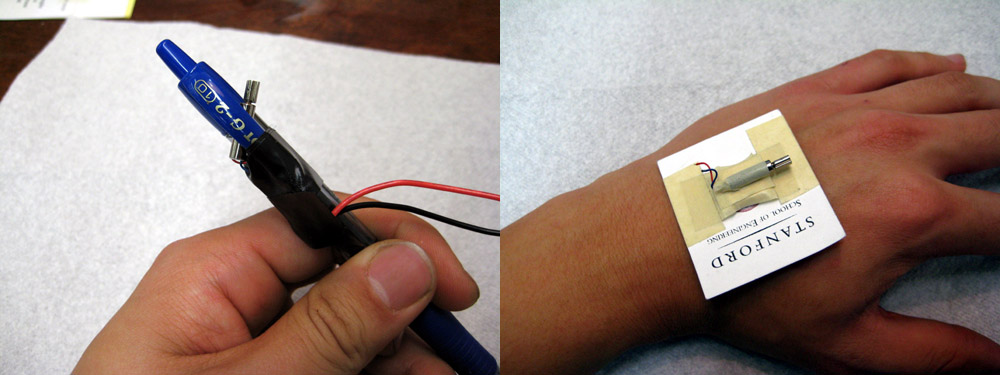
\includegraphics[width=0.8\textwidth]{Figures/Ch4/tactile_motor.jpg}
	\caption[Messaging station wires]{The orientation of the two tactile messaging stations. (Note: the wires connecting the patch to power supply are not in this photo)}
\end{figure}

	The tactile messaging critical function prototype was a success in that it definitively answered all the critical questions we asked ourselves before testing.
   %Results of benchmarking, need-finding, CFP, CEP etc.

%%%%%%%%%%%%%%%%%%%%%%%%%%%%%%%%
\chapter{Design Vision}
%\chapter{Design Description}   %This title will make more sense in Winter and Spring.
\label{design-description}

This \textbf{Design Description} chapter defines what the design is. But for Fall, it's really your vision or proposal for what you think the design might be by the end of Winter or Spring quarter. So let's call it the \textbf{Design Vision} chapter in Fall. It will be a short
chapter. 

Even so, on the basis of preliminary need-finding, benchmarking and critical function evaluation, you should have some idea of what may be appropriate. Take a point of view and assert it!  A CAD rendering, a systems diagram or even a sketch of a concept could help to explain your vision. 

If you find yourself adding rationale, or discussing design alternatives or how the vision came about, you are writing text that should be moved into the end of the Development section. This is section is about what the design (or vision) 
is, not how it came to be.

\begin{remark}\color{blue}
\section{Vision}
\label{vision}

For Winter and Spring, although you now have a design to describe, you probably want to start off your Design Description chapter with a reminder of the overall vision, toward
which your current design is an important intermediate step.

Use this section to describe your vision or proposal for what you think the design might be. Ideally you should have a sketch, a diagram or other images to help define it.  
\section{Specifications}
\label{specifications}

In Winter and Spring here is where you describe what your design is. 
\begin{itemize}
\item Define the subsystems and how they go together.
\item Use diagrams, CAD renderings, tables, etc. to make it clear. 
\item Use flow charts or pseudocode to describe procedures.
\item Detailed source code and numerical data should go in an Appendix section or, if really long, on a CD or other electronic format (nobody will wade through the printout).
\end{itemize}

\normalcolor\end{remark}





  %This section is just your proposal or "Vision" for Fall.

%%%%%%%%%%%%%%%%%%%%%%%%%%%%%%%%
\chapter{Planning}
\label{project-planning}

\begin{remark}\color{blue}
Teams with global partners face special challenges in  terms of organization, project management and planning.
It is a truism that organizational burden goes as the square of team size. 

To address these issues, we ask each local+global team to prepare a \textbf{plan for Winter quarter} to include in this section. You have just accomplished a first, rough critical function prototype (CFP and CEP) and you have given a presentation and written a document that captures the current state of your vision and findings. You have learned who can do what and how much work it really takes. And you are highly motivated to make Winter go more smoothly and to ``take control'' of your project.
\normalcolor \end{remark}

\section{Deliverables}
Define briefly what will be delivered. Of course, this is to the best of your current knowledge -- things will change. A short table with some explanatory text could be used here. Your project plan should include the following non-negotiable items and any sub-tasks or intermediate items'' that lead up to them. Consult the course calendar for dates and more details.

\begin{itemize} \tightlist
\item Travel: When are you traveling? What is planned for the trip?
\item Dark Horse prototype -- a 2nd CFP that probes the edge of the design space
\item Travel Docs due
\item Funky Prototype -- an initial system where a potential avenue for the final product is developed
\item Functional System Review -- your latest and greatest as Winter quarter draws to a close. It should give a clear indication of what to confidently expect in June.
\item Winter Design Documents
\end{itemize}

\section{Milestones}
When are various elements (e.g., rough prototypes, final prototypes) delivered? When are key tests conducted? These are the dates, times, and places where project progress is observable and/or demonstrated. Again, update with planned versus actual dates as the design progresses.

\section{Distributed Team Management}
Explain how your distributed and interdisciplinary team will collaborate, communicate and keep itself on-track with respect to the afore-mentioned deliverables.

\section{Project Budget}
As with any serious proposal, you should include an estimated budget with some specifics about money that has been spent (Fall) and probably will be spent (Winter). Details on vendors can be put in the Appendix. A common mistake is that teams spend too little money until late in the quarter and then spend too much, doing rush jobs and rework.

\section{Project Time Line}
Summarize the projected project time line if it is not already explicit in the project planning representations above.

Use any of the familiar project development representations including lists, Gantt Charts, Pert Charts (Figure \ref{fig:full-page-example}), bubble diagrams, tables, etc. In addition, you will almost certainly need a list or table of items that says a bit
more about the items and gives an idea who is going to do what.

\begin{figure}[bhtp] 
\centering
		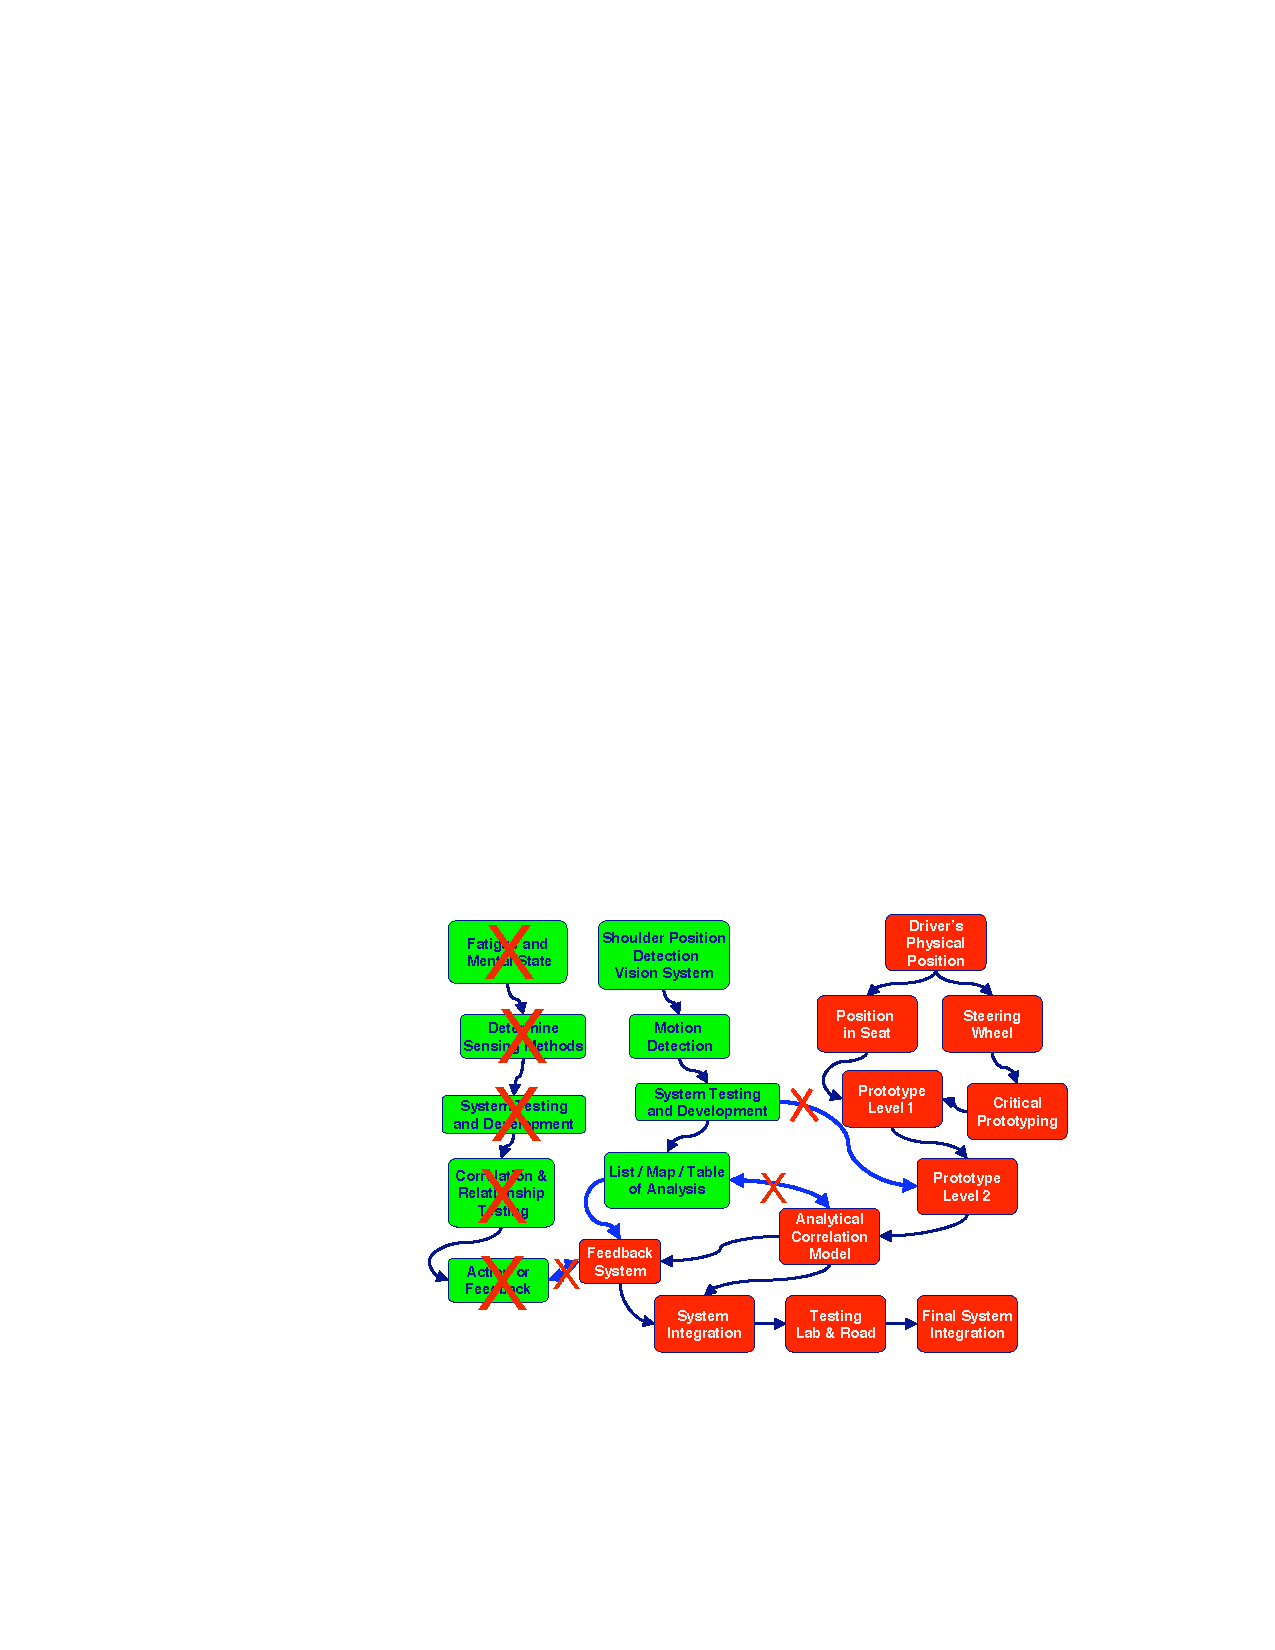
\includegraphics[width=\textwidth]{Figures/Ch6/su-tmit-after.pdf}
	\caption[Project task replanning example]{In this example from \cite{Toyota01}, Stanford students collaborated with a group at TMIT, Japan. At the end of the Winter quarter it was decided to abandon one branch of the TMIT effort and to eliminate some of the tight coupling that was originally envisioned. }
	\label{fig:su-tmit}  %Tag for referring to figure in text.
\end{figure}

\begin{figure}[p]   % p for "page" for let it be a full page figure!
\centering
		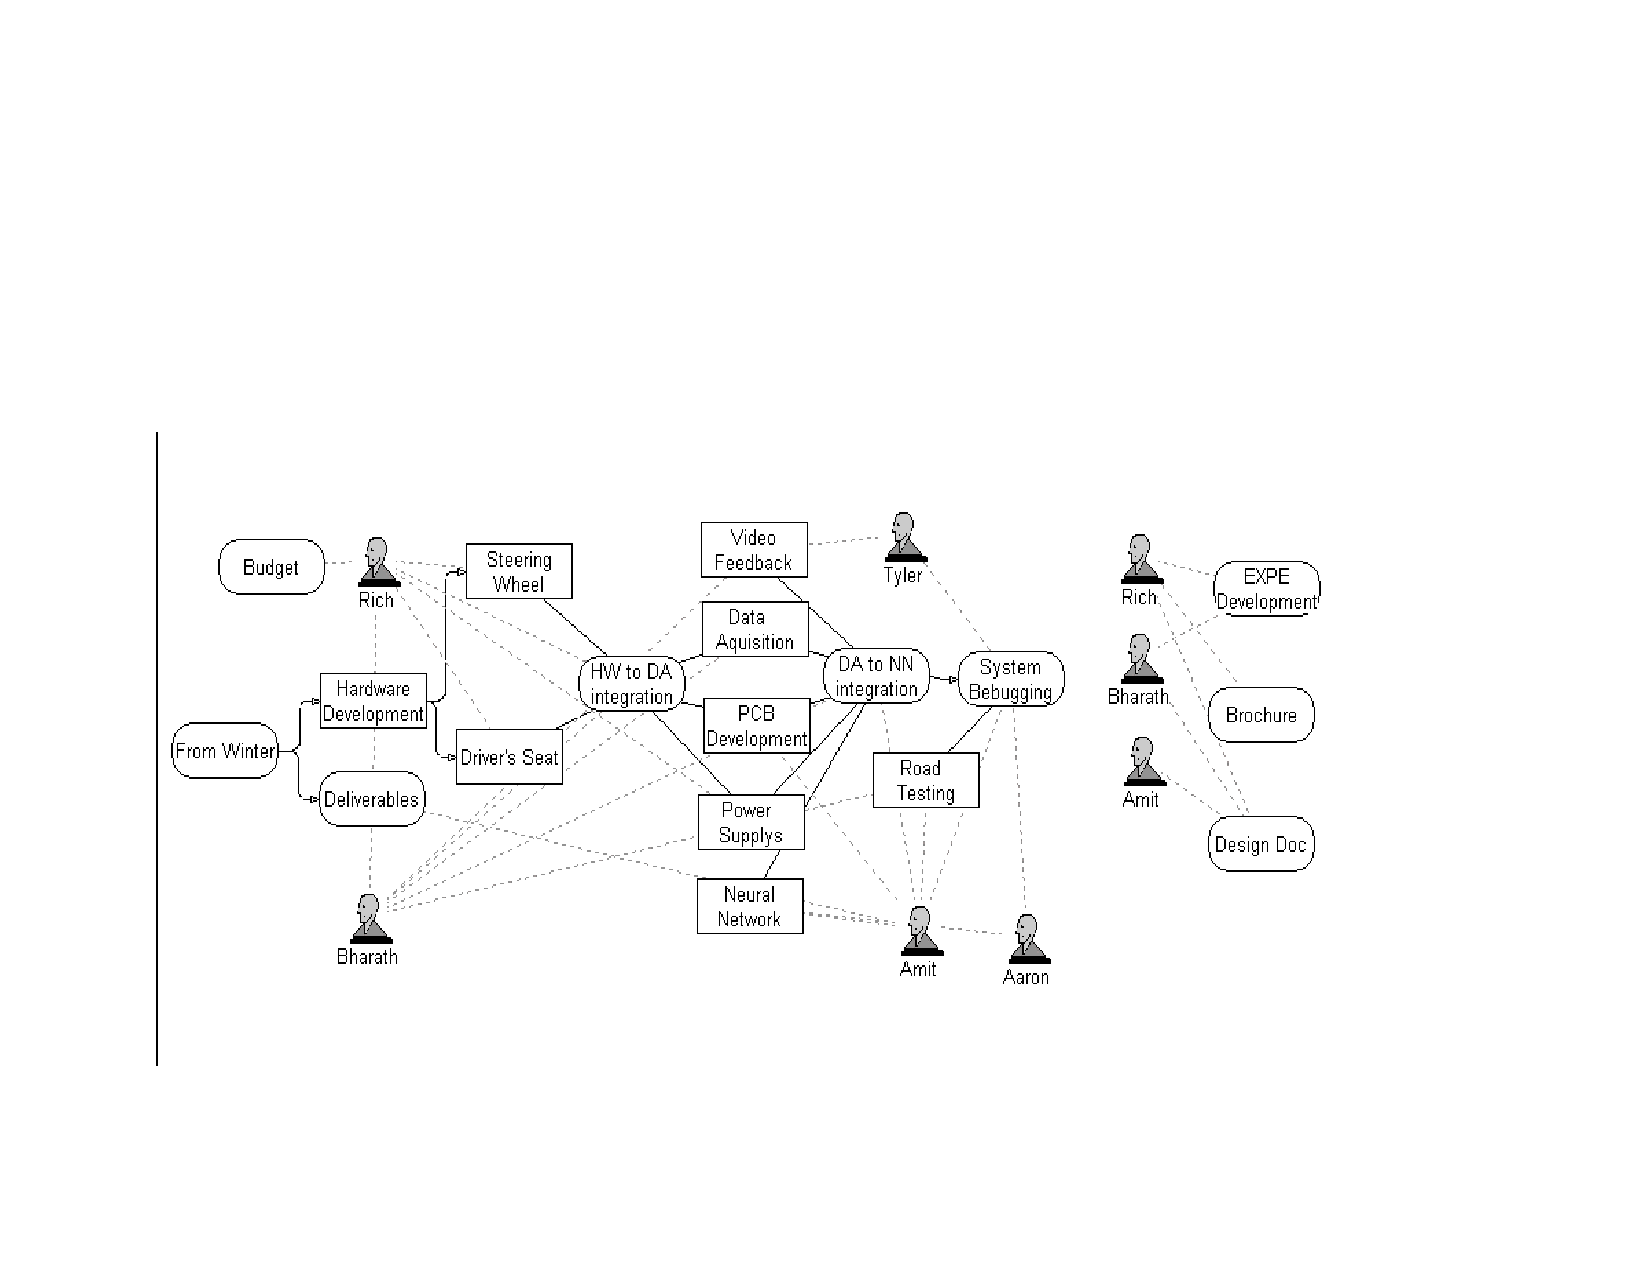
\includegraphics[angle=90, height= 8in]{Figures/Ch6/ideastorm}
	\caption[Rotated landscape figure example]{An example of taking a large figure and having Latex rotate it 90 degrees to display it in landscape format as a full page figure.}
	\label{fig:full-page-example}  %Tag for referring to figure in text.
\end{figure}

\section{Reflections and Goals}
This is the one section that you would not find in normal research or engineering proposal. But in the spirit that we're doing this in an academic setting, we want to be sure that we reflect on what we're learning and thinking and where we hope to go with it. The reflections are personal, and can be written diplomatically, for example using the \emph{I like..., I wish...} protocol.

A part of reflective section may include how your team functioned in the fall - explaining how and why your actual design process deviated from what you originally planned, if relevant. (Time lines and milestones often have the look of having been concocted the night before the report is due.)
  %Current and future plans.

%%%%%%%%%%%%%%%%%%%%%%%%%%%%%%%%
% Appendices are set up same as chapters
\chapter{Resources}
\label{cha:resources}

Include lists of human, institutional and vendor resources here with contact information. This is not for direct citations, which go on the Bibliography.  

%%%%%BEGIN BIBLIOGRAPHY%%%%%%%%%
% This is a two-step process in which you first create a ".bib" file, which is processed
% by bibtex into a ".bbl" file for loading into the document. 
% Many online journals and databases now have a feature to automatically download Bib
% citations.  BibDesk is a handy (free) program for Macintosh for managing them.
% EndNote and Refworks (is free to Stanford students) are good alternatives.
\bibliographystyle{plainurl310}     %Modified slightly from plainurl.bst 
\bibliography{me310reportfall}  % Look for file called "me310report.bib" 
%
% Alternatively, you can create your own bibliography list by hand.
% In that case, comment out the last line above and replace with  \input{OurBibFile} 
%%%%%END BIBLIOGRAPHY%%%%%%%%%

%%%%%BEGIN APPENDIX SECTIONS%%%%%%%%%%%%%%%
\begin{appendices}
 % Appendices are set up same as chapter sections
\chapter{Appendices}

\section{User Survey Responses}
\label{sec:AppendixSurvey}


\includepdfmerge[nup=2x2]{survey/Response1, 1-5, survey/Response2, 1-5, survey/Response3, 1-5}


       % There could be multiple appendix files like this
 \end{appendices}
 %%%%%END APPENDIX SECTIONS%%%%%%%%%%%%%%%
 
\end{document}

